\documentclass[11pt]{article}

% Packages
\usepackage[utf8]{inputenc}
\usepackage[T1]{fontenc}
\usepackage{amsmath}
\usepackage{amsfonts}
\usepackage{amssymb}
\usepackage{amsthm}
\usepackage{graphicx}
\usepackage{url}
\usepackage{hyperref}
\usepackage{geometry}
\usepackage{natbib}
\usepackage{array}
\usepackage{booktabs}
\usepackage{subcaption}

% Page setup
\geometry{margin=1in}
\linespread{1.2}

% Theorem environments
\newtheorem{definition}{Definition}
\newtheorem{corollary}{Corollary}

\title{Consciousness and Unambiguous Representations}

\author{Francesco Lässig}

\date{\today}

\begin{document}

\maketitle

\begin{abstract}
Impure representationalism (Chalmers, 1996) is one proposal for tackling the Hard Problem of consciousness: it identifies phenomenal properties with the right manner of representation. However, what counts as right remains underspecified, leaving a key gap in determining the conditions a representation must satisfy. I suggest that a necessary ingredient is unambiguity: ruling out competing interpretations. I model ambiguity as the entropy of interpretations given a representation and estimate it in artificial neural networks. Using a relational decoder that sees only similarity patterns among shuffled neurons in unseen MNIST classifiers, I test whether these patterns alone reveal what neurons are about.

Main findings: (1) Relational structure generalizes across networks. The decoder recovers what neurons represent (e.g., class identity or pixel location) in new models purely from inter-neuron relations. (2) Training choices modulate ambiguity. Networks with nearly identical input-output accuracy differ sharply in estimated ambiguity, indicating that ambiguity is largely independent of task-level performance.

By turning ambiguity into a measurable quantity, the relational decoder paradigm not only operationalizes the ``right manner'' clause of impure representationalism but, whereas most current theories focus on quantifying the level of consciousness (e.g., IIT's $\Phi$), it also offers a computational handle on the contents of consciousness.
\end{abstract}

\section{Introduction}

The relationship between neural activity and conscious experience remains one of the most challenging problems in cognitive science. While representational theories suggest that conscious experiences correspond to neural representations, this framework faces a fundamental challenge: most representations are inherently ambiguous without appropriate decoding schemes. A bit string can represent an image, sound, text, or any digital medium depending on how it is decoded. Similarly, patterns of neural activity could potentially represent different conscious experiences under different interpretations.

This ambiguity problem becomes particularly acute when we consider that conscious content appears to be determined in each moment of experience. When we see an apple, the content of our visual experience is about an apple specifically, not about oranges or sounds or any other possible interpretation. This determination occurs without requiring us to consciously apply a decoding scheme or compare our current experience against all possible alternatives.

In this paper, we address this challenge by proposing that conscious representations must be fundamentally unambiguous. In other words, they must intrinsically specify both their content and their interpretation. We develop a formal framework for measuring representational ambiguity and demonstrate how neural networks can develop such unambiguous representations through learning processes.

\section{Theory}

\subsection{Ambiguous Representations}

Representations are ubiquitous within our daily lives: letters represent sounds, words represent concepts, bit strings represent files. However, these representations are only meaningful insofar as they are decoded in the right way. Roman letters are meaningless to someone only familiar with Chinese characters, the word `Utangatta' is only meaningful if you know Icelandic, and a bit string representing a JPEG image of an apple only does so if the right decoding algorithm is applied.

Given the right decoding algorithm, the same bit string could be decoded into a sound file, a video game, a text, or any other type of digital medium. Generally speaking, there is no information inherent in a bit string that tells us anything about what it is about. For all examples provided so far, this does not pose a problem. Representations such as letters, words and bit strings are useful because we can agree on decoding schemes that should be applied for a given set of representations.

Representations in conjunction with an encoding scheme bear meaning, thus rendering them useful to us. Without an encoding scheme, however, most representations are ambiguous: they could represent anything.

\subsection{Representational Accounts of Consciousness}

One strategy to think about a mapping between neural activity and conscious experience is in terms of a representational relationship \cite{lycan2019}. If I see an apple, neural activity in my brain is representing an apple. This idea of a representational relationship accounts for the fact that the experience of an apple is not dependent on the presence of the actual apple in the real world. After all, dreams and hallucinations of apples are real phenomena.

If conscious experience corresponds to the presence of representations, dreams of apples can be explained as instantiating a representation in the absence of the actual apple in the real world. But this begs the question of what encoding scheme is used to represent the visual perception of an apple in terms of neural activity.

\subsection{Conscious Content is Determined}

It is reasonable to assume that a brain in a given state has a determined conscious experience (or a determined set of conscious experiences to allow for the case of islands of consciousness that could conceivably occur in healthy individuals or perhaps more likely in split brain patients \cite{bayne2020}). In any case, a given brain state that is postulated to account for a given experience cannot at the same time account for a different, conflicting experience.

In other words, if I see an apple, then part of my brain is representing an apple, and the same neural activity is not also representing an orange, or the sound of a passing car (which could concurrently be represented, but not alternatively decoded instead of decoding the apple). This is arguably already the case prior to any higher cognitive judgements about the nature of the experience, as the appearance of the apple itself already presupposes what it is about.

Not only does it presuppose it's about an apple, but it presupposes it's about something visual. Acting upon the correct identification of the object is not necessary for postulating that a representation has determined content. This is because, while the content of consciousness certainly guides our behavior, it is arguably not dependent on it.

\subsection{Conscious Content is Not Determined by a Decoder}

Given what we know about the nature of bit string encodings of images and similar representations, it might be tempting to propose a decoder within our brain that gives meaning to our representations of the real world. If we follow this line of reasoning, it would be our `internal decoder' that is responsible for conscious experience, since only when decoded do representations become meaningful.

But all a decoder can do is to transform representations in one encoding to a different encoding. We are still left with the question of how this new encoding `knows' what it is about, or, in other words, why this representation is about one specific thing (an apple) as opposed to anything else. Postulating a special brain area that reads out the meaning of representations is just an instance of the internal homunculus or Cartesian theater fallacy \cite{pennartz2022}.

\subsection{Conscious Representations are Unambiguous}

If the content of conscious representations is determined, and if we can't rely on a decoder to give it meaning, we must assume that, unlike for bit strings or letters, the encoding intrinsically carries meaning about the intentional content of the representation. This gives us a formal requirement for a conscious representation.

\begin{definition}[Intentionality Constraint]
The intentionality constraint on NCCs requires that an explanatory NCC of an aspect of conscious experience must unambiguously represent that aspect.
\end{definition}

\begin{corollary}
Conscious representations need to carry meaning about how they are representing things in addition to what they are representing.
\end{corollary}

To illustrate the strength of this constraint, let's consider again the JPEG. While the meaning of a bit string representing a JPEG image is ambiguous and meaningless by itself, given enough pairs of bit strings and images, one could deduce the decoding, and thus the meaning of the individual bit string. However, the contents of consciousness of a subject are already determined within one moment (again, subject to microgenesis constraints).

There is no need for some external observer to scan the subject's brain in many different states to give meaning to the current conscious representations. To the brain itself, they carry meaning, i.e., represent a determined conscious experience, in every moment.

Note that I'm proposing that this intentionality constraint is a necessary, but not necessarily sufficient condition for phenomenal consciousness. While an unambiguous representation might have clear intentional content to an outside observer, this content might not `appear to itself'. We might have to postulate additional requirements, such as `integration' for consciousness to arise.

\subsection{Defining Ambiguity}

An unambiguous representation conveys content as well as how to decode that content, thus leaving us with only one possible interpretation. On the other hand, a representation is ambiguous to the extent that it does not exclude other possible interpretations. To allow for a spectrum of ambiguity levels, with completely ambiguous representations such as random bit strings on the one hand, and completely unambiguous conscious representations on the other, we propose the following formalism:

\begin{equation}
\text{Ambiguity} = H(I|R)
\end{equation}

where $H$ denotes the entropy function and $I|R$ the probability distribution of all possible interpretations given a certain representation. Of course, despite the mathematical formulation, without further assumptions this is not a computable quantity. In addition to the set of interpretations being intractable, the relationship between representations and possible interpretations is not clear, although relation-preservation might be a good candidate \cite{kleiner2024}.

Still, this definition of representational ambiguity should help the reader get a sense for what I mean with `ambiguity'.

To illustrate this formulation with a concrete example, consider a simple case where a representation $R$ can have three possible interpretations $I = \{i_1, i_2, i_3\}$. For a completely ambiguous representation (like a random bit string), the conditional probability distribution would be uniform: $p(i_1|R) = p(i_2|R) = p(i_3|R) = 1/3$, yielding $H(I|R) = \log_2(3) \approx 1.58$ bits.

For a partially unambiguous representation that strongly suggests one interpretation over others, we might have $p(i_1|R) = 0.7$, $p(i_2|R) = 0.2$, $p(i_3|R) = 0.1$, yielding $H(I|R) = 0.9$ bits. Finally, for a completely unambiguous representation like those postulated for consciousness, we would have $p(i_1|R) = 1$, $p(i_2|R) = p(i_3|R) = 0$, yielding $H(I|R) = 0$ bits.

This illustrates how the ambiguity measure captures the uncertainty about the correct interpretation given a representation.

\subsection{Relational Structures as Unambiguous Representations}

How could any type of encoding convey meaning without presupposing a decoding scheme? We saw that a bit string cannot do the job. The reason for that is that it is a purely indexical object. A bit string is a number, and all it tells us is that it is this number and not any other number. What we need is structure.

Let's illustrate this using an example. Let's say we encode a $5 \times 5$ image of a square by encoding all the values of the individual pixels, giving us a 25-dimensional vector (Figure \ref{fig:pixel-encoding}a). While this looks to us like it is representing a square, this is only true because we have arranged the values of the vector in the appropriate way. The information about how the vector should be decoded is not contained within the vector itself.

However, if in addition to the vector, we include a set of relations to our representations that link neighboring vector elements, then the read-out of the vector as a square grid ceases to be arbitrary (Figure \ref{fig:pixel-encoding}b). Essentially, we give every vector element a meaning by defining how it relates to other vector elements. The values of the vector lose their arbitrariness to some extent.

\begin{figure}[htbp]
\centering
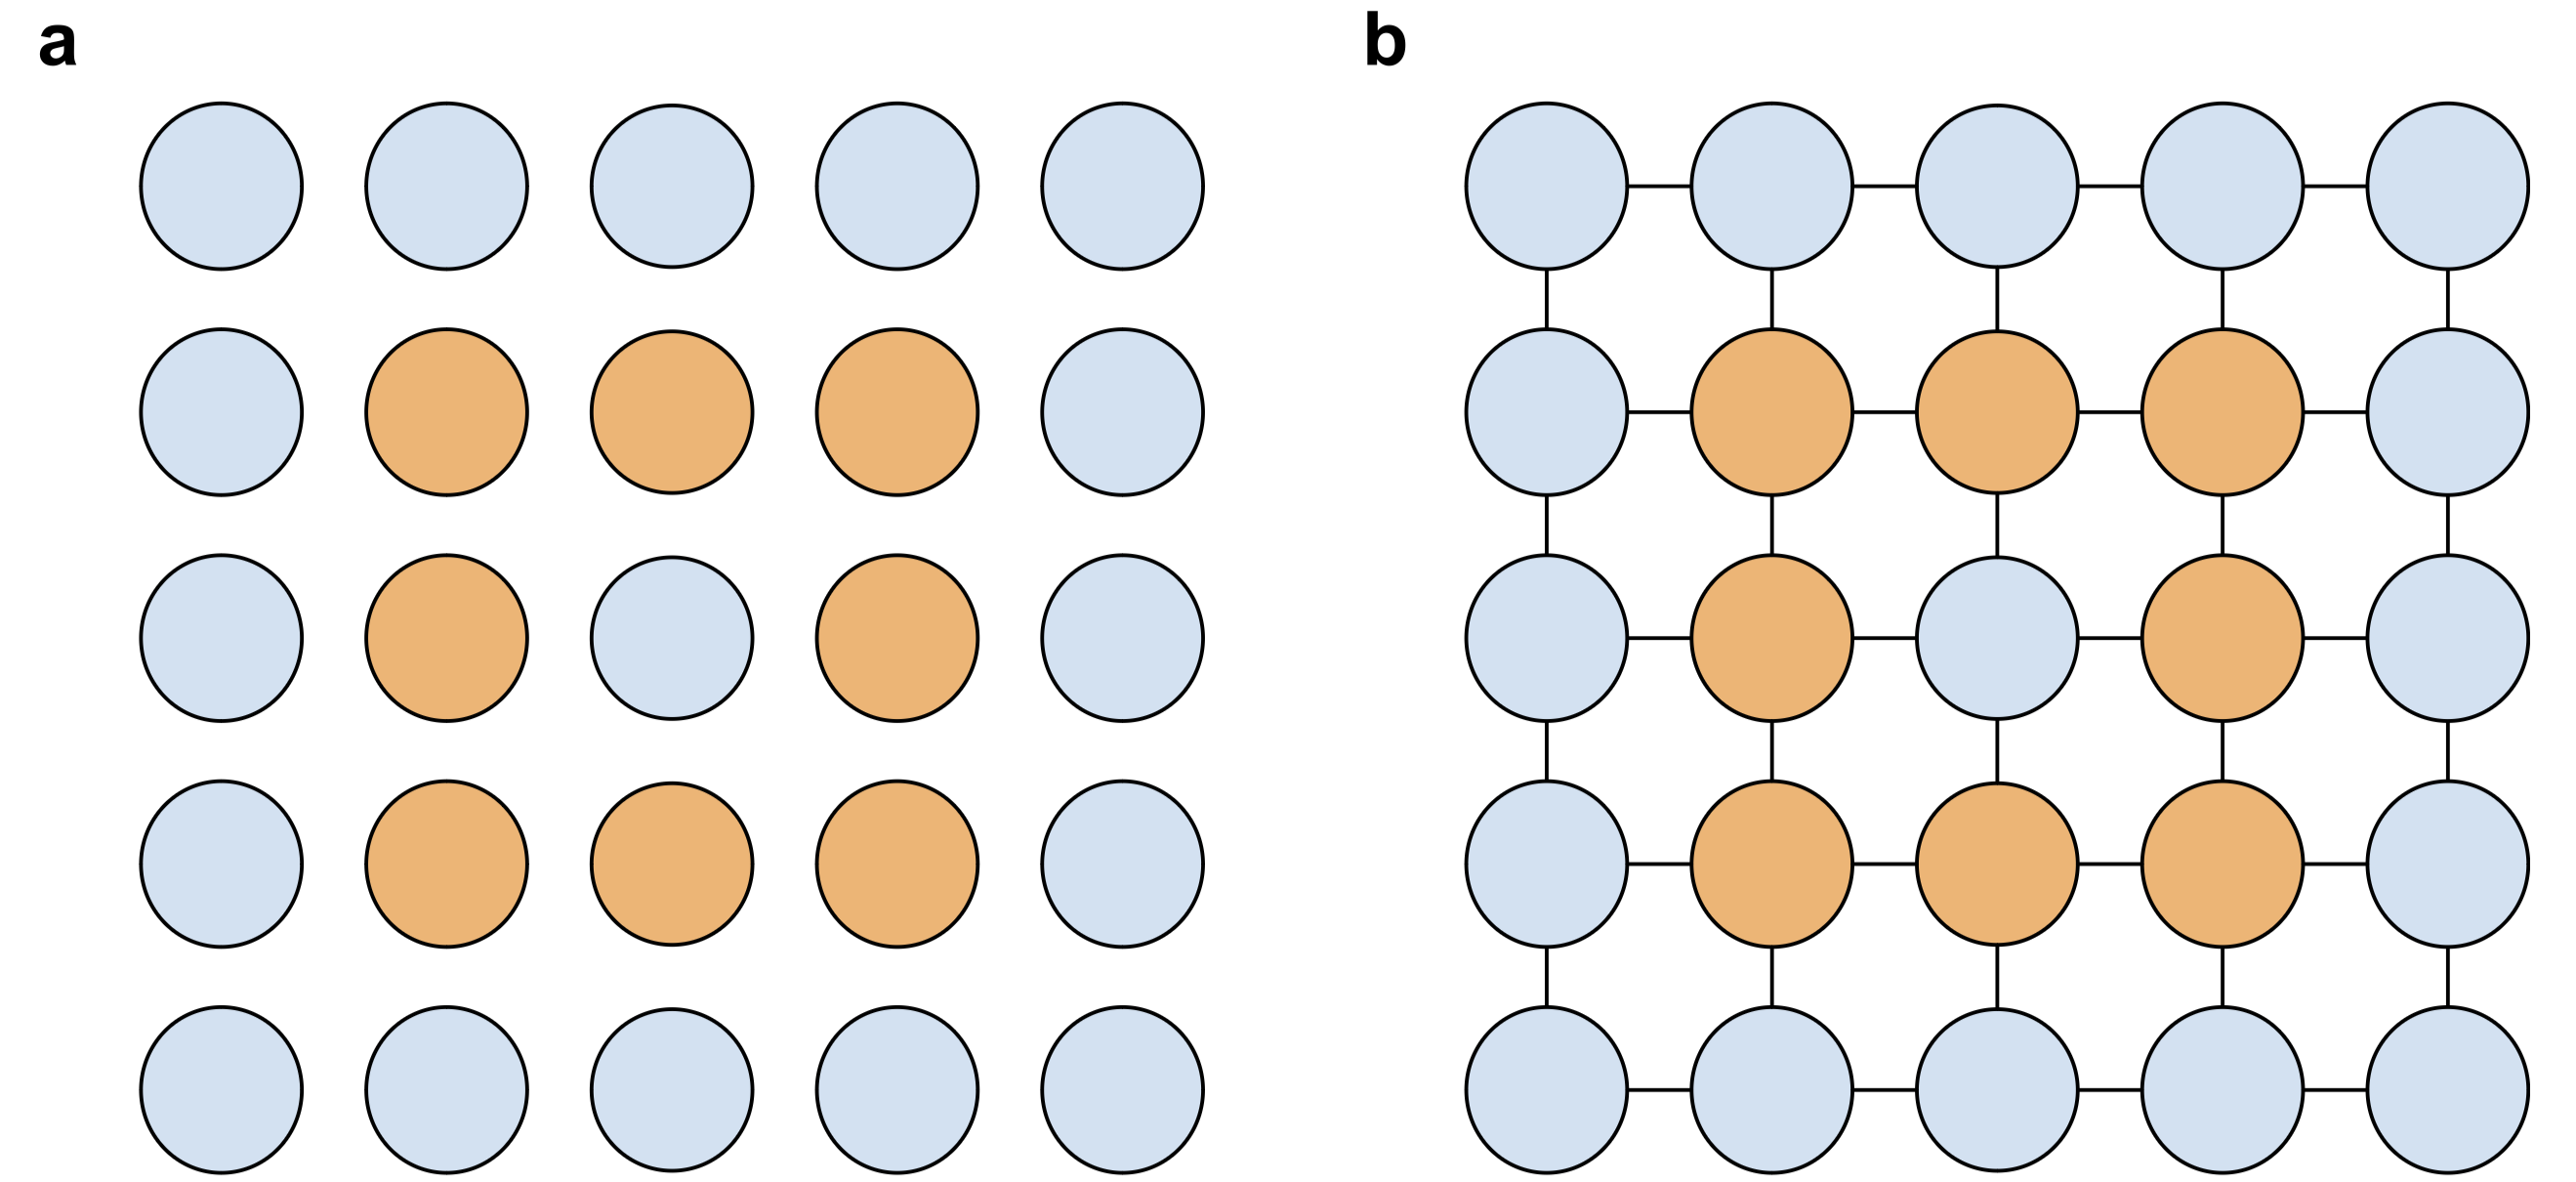
\includegraphics[width=0.8\textwidth]{figures/pixel-encoding-relational-structure.png}
\caption{Pixel encoding and relational structure: \textbf{(a)} Visualization of the elements of a binary vector (orange=1, blue=0) as a square grid. \textbf{(b)} Set of relations between neighboring vector elements in addition to the vector elements themselves.}
\label{fig:pixel-encoding}
\end{figure}

Note that I am not claiming that this structure can account for the richness of spatial experience \cite{haun2019}, but it can restrict the space of possible decodings to some extent, giving rise to the possibility of unambiguously decoding something like a square.

Consider a musical major chord as an analogy for unambiguous relational structures. The identity of a `major chord' emerges not from its individual notes but from their specific intervallic relationships (root, major third, perfect fifth). C-E-G, D-F\#-A, and F-A-C are all recognized as major chords despite having different constituent notes because they maintain the same relational pattern.

This structure gives each chord its characteristic `major' quality that remains invariant across different keys. Similarly, neural networks may encode meaning through invariant relational patterns that persist despite variations in specific activations.

\subsection{Two Types of Structuralism}

Within the field of consciousness research and philosophy of mind, the idea of conscious experience being determined relationally is known as structuralism \cite{lyre2022}. However, it is important to note two types of structuralism:

\begin{enumerate}
\item The content of an experience is determined by its relation to all other possible experiences that a subject could have had.
\item The content of an experience is determined by relations instantiated in the current moment.
\end{enumerate}

In both consciousness science and philosophy of mind literature, structuralism is often understood in the first sense \cite{lyre2022}. However, this does not address the intentionality constraint because conscious experience is already determined in one moment. It is not clear how the mere potentiality of other experiences and their relations to the current one could actively determine the character of the current conscious experience.

What I am suggesting is that conscious experience is determined in the second sense, i.e., by a relational structure that is instantiated in the current moment. It is quite possible that these two types of structuralism map onto each other somehow. Structuralism 2 might in some way be a mirror image or a consequence of structuralism 1. Nevertheless, to determine the character of the current experience, it is the second one that counts.

\subsection{Structure of Conscious Experience Must Emerge Unambiguously from Substrate}

Even if the proposed mathematical structure of experience encodes meaning intrinsically, the way this structure is obtained from the (neural) substrate cannot be arbitrary. If we need an arbitrary decoding algorithm to obtain our mathematical structure from the substrate, we again run into the problem of why this particular decoding scheme is used as opposed to any other. To avoid this, we need to unambiguously tie the relational structure to physical reality.

In the following we list some potential requirements for this `physical grounding' of relational structures corresponding to conscious representations:

\begin{enumerate}
\item \textbf{Temporal continuity of encoding.} The way elements and relations of the mathematical structure representing conscious content are implemented in the physical substrate need to stay consistent over time. To consider a silly example, let's say two elements of our relational structure are grounded in two carbon atoms, and that a relation relevant to the structure of the conscious experience of that system is grounded in a covalent bond of that structure. The fact that atoms ground elements and covalent bonds ground relations needs to stay consistent.

\item \textbf{Correspondence of concrete physical entities with elements of mathematical structure.} Elements in a relational structure representing conscious contents need to correspond to physical `objects' that can be delineated from the rest of the universe by some objective measure. Otherwise, there remains inherent ambiguity about what the elements and relations of our structure are.

\item \textbf{Physically meaningful connection between relations and elements of mathematical structure.} Going back to our example of the carbon molecule, if two elements of a relational structure are grounded in two C atoms, then a relation between the two should be grounded in a physical quantity/object that relates the two carbon atoms. If the relation between the two elements grounded in the C atoms were grounded by a covalent bond in a different molecule, there would be inherent ambiguity about which relations link which elements of the relational structure.
\end{enumerate}

Overall, ambiguity in a representation can arise at two stages:
\begin{enumerate}
\item The abstract mathematical representation is inherently ambiguous (for instance a bit string).
\item The way physical substrate implements this mathematical representation is ambiguous, i.e., although the abstract mathematical representation is intrinsically meaningful, it is not unambiguously decodable from the substrate.
\end{enumerate}

\subsection{Neural Networks as Mathematical Structures of Consciousness}

Relational structures can give meaning to elements of a representation by defining how they are related to other elements. But what kind of relational structure might be dictating the contents of our consciousness? To answer this question, let's return to the example of an image represented as a pixel vector.

As mentioned previously, there is no way of knowing what a specific vector $v$ is about, without being provided with the encoding scheme used. However, given the full distribution of natural images $X \sim p(x)$, we could conceivably deduce that the vectors encode something 2D (this could be achieved by noticing strong correlations between vector elements corresponding to adjacent pixels and deducing the grid from that), and additionally, we could probably decode and visualize vector $v$, which is one sample of $X$.

Does this make intentionality trivial? Not in the case of conscious representations. This is because a single conscious experience is already determined in the moment we are experiencing it. It doesn't have to be compared against the whole distribution of other possible conscious experiences, at least not explicitly. After all, to see a square, we don't have to see all possible arrangements of edges and shapes to make sense of that experience.

However, implicitly we may make use of exactly this information. Through evolution and plasticity, our brain has learned to model real-world distributions in its neural circuitry. While this model only represents one, say, visual experience at any given moment, it embeds this representation within a network that models the structure of the whole distribution of all visual experiences encountered in the natural world.

This way it re-instantiates the whole distribution when experiencing a single instance of it, thus giving it meaning. Essentially, by mirroring the distribution of the natural world (which involves modeling its relations), a neural network can not only unambiguously encode a mathematical structure corresponding to contents of consciousness, but the network itself might be a candidate for a mathematical structure of consciousness.

\section{Exhibit 1: MNIST Digit Representations}

\subsection{Experimental Design}

In this experiment we illustrate how artificial neural networks can unambiguously represent inputs by capturing characteristics of the input distribution in their connectivity. We propose the following task: for an unseen network trained to classify MNIST images, we want to deduce the class that a given output neuron encodes, with no guarantee about the order in which the output neurons are given.

Moreover, we want to decode the class of a given neuron purely based on the connectivity of the output layer to the previous layer. The idea is that the connectivity of the network allows us to identify a relational structure between the output neurons that reflects characteristics of the MNIST distribution. Within this relational structure, we hypothesize that each MNIST class occupies a unique position relative to the other classes.

\subsection{Machine Learning Setup}

To operationalize this idea, we want to turn it into a machine learning problem: can we train a decoder that predicts the class of an output neuron purely based on connectivity of the output layer to the previous layer? Note that we cannot train the decoder on the same network it should be evaluated on, since that would result in the decoder learning a network-specific mapping of neurons to classes, and not a general principle of aboutness for MNIST.

To avoid this, we train many networks using different random seeds on MNIST to generate the training and validation data. Crucially, data from the same network is only contained in either the training or the validation set, but not in both. This way, the only way for the decoder to solve the task is to learn to recognize consistent patterns in connectivity across different networks that are informative about class identity.

\subsection{Dataset Construction}

To train a decoder to predict which class a given output neuron represents based on the incoming weights to the output layer, we construct an input-output pair $(X, y)$ in the following way: for a given network that was trained on MNIST, let $W$ denote its output layer weights. We define $X$ as a matrix consisting of a random permutation of the rows of $W$.

This means that each row of $X$ corresponds to the input weights of one of the output neurons of the underlying network. Moreover, any row of $X$ could be associated with any of the output neurons of the underlying network, and thus with any of the 10 MNIST classes. Finally, we define $y$ as the class index of whichever output neuron ended up being the first row of $X$.

Thus, what the decoder `sees' is a set of weight vectors corresponding to output neurons of the network. The position of these vectors within $X$ contains no information, except that the decoder will have to predict the class index of the one that occupies the first row.

To generate a dataset for one type of MNIST-classifying network, we train the underlying network on 1000 different random seeds, resulting in 1000 sets of output layer weights. Since each network has 10 output neurons, this gives us a total of 10,000 data points, one for each output neuron across all trained networks.

\subsection{Preprocessing}

While the dataset we described above should contain all the information the decoder needs to predict the class of an output neuron by identifying its relations to other output neurons, in practice we found that the decoder does not naturally learn to identify these relations well. To point the decoder in the right direction, we applied the following preprocessing step to $X$:

\begin{align}
X_{\text{norm}} &= \frac{X}{\|X\|_{\text{row}}} \\
X' &= X_{\text{norm}} X_{\text{norm}}^T \\
(X')_{i,j} &= \frac{X_i \cdot X_j}{\|X_i\| \|X_j\|}
\end{align}

Where $X_i$ denotes the $i$-th row of $X$, $\|\cdot\|_{\text{row}}$ denotes row-wise L2 normalization, and $\cdot$ represents the dot product. Like $X$, the rows of $X'$ all correspond to one of the output neurons and the first row corresponds to the output neuron whose class index should be predicted by the decoder.

However, instead of representing the incoming weights of an output neuron, a row now represents the cosine similarities between that neuron's incoming weights with all other output neurons' incoming weights. In other words, the value $(X')_{i,j}$ represents the cosine similarity between the incoming weights of output neuron $i$ and output neuron $j$.

\subsection{Decoder Architecture}

Because the order of the rows of $X'$ beyond the first row (which always corresponds to the output neuron whose class should be predicted) contains no useful information to solve the task, we want our decoder to be invariant to permutations of the rows of $X'$. We achieve this using a Transformer-like architecture with self-attention layers \cite{vaswani2017}, as seen in the decoder architecture pipeline below (panel d).

We treat the rows of $X'$ as tokens, pass the data through two multi-head self-attention layers and finally read out the result from the first token's learned representation using a linear layer that produces a 10-dimensional output. During training, we compute the cross entropy loss between this output and the label $y$. To compute the validation accuracy, we simply take the output of the decoder with the highest value as our class prediction for a given data point. Figure \ref{fig:decoder-architecture} shows the whole architecture.

\begin{figure}[htbp]
\centering
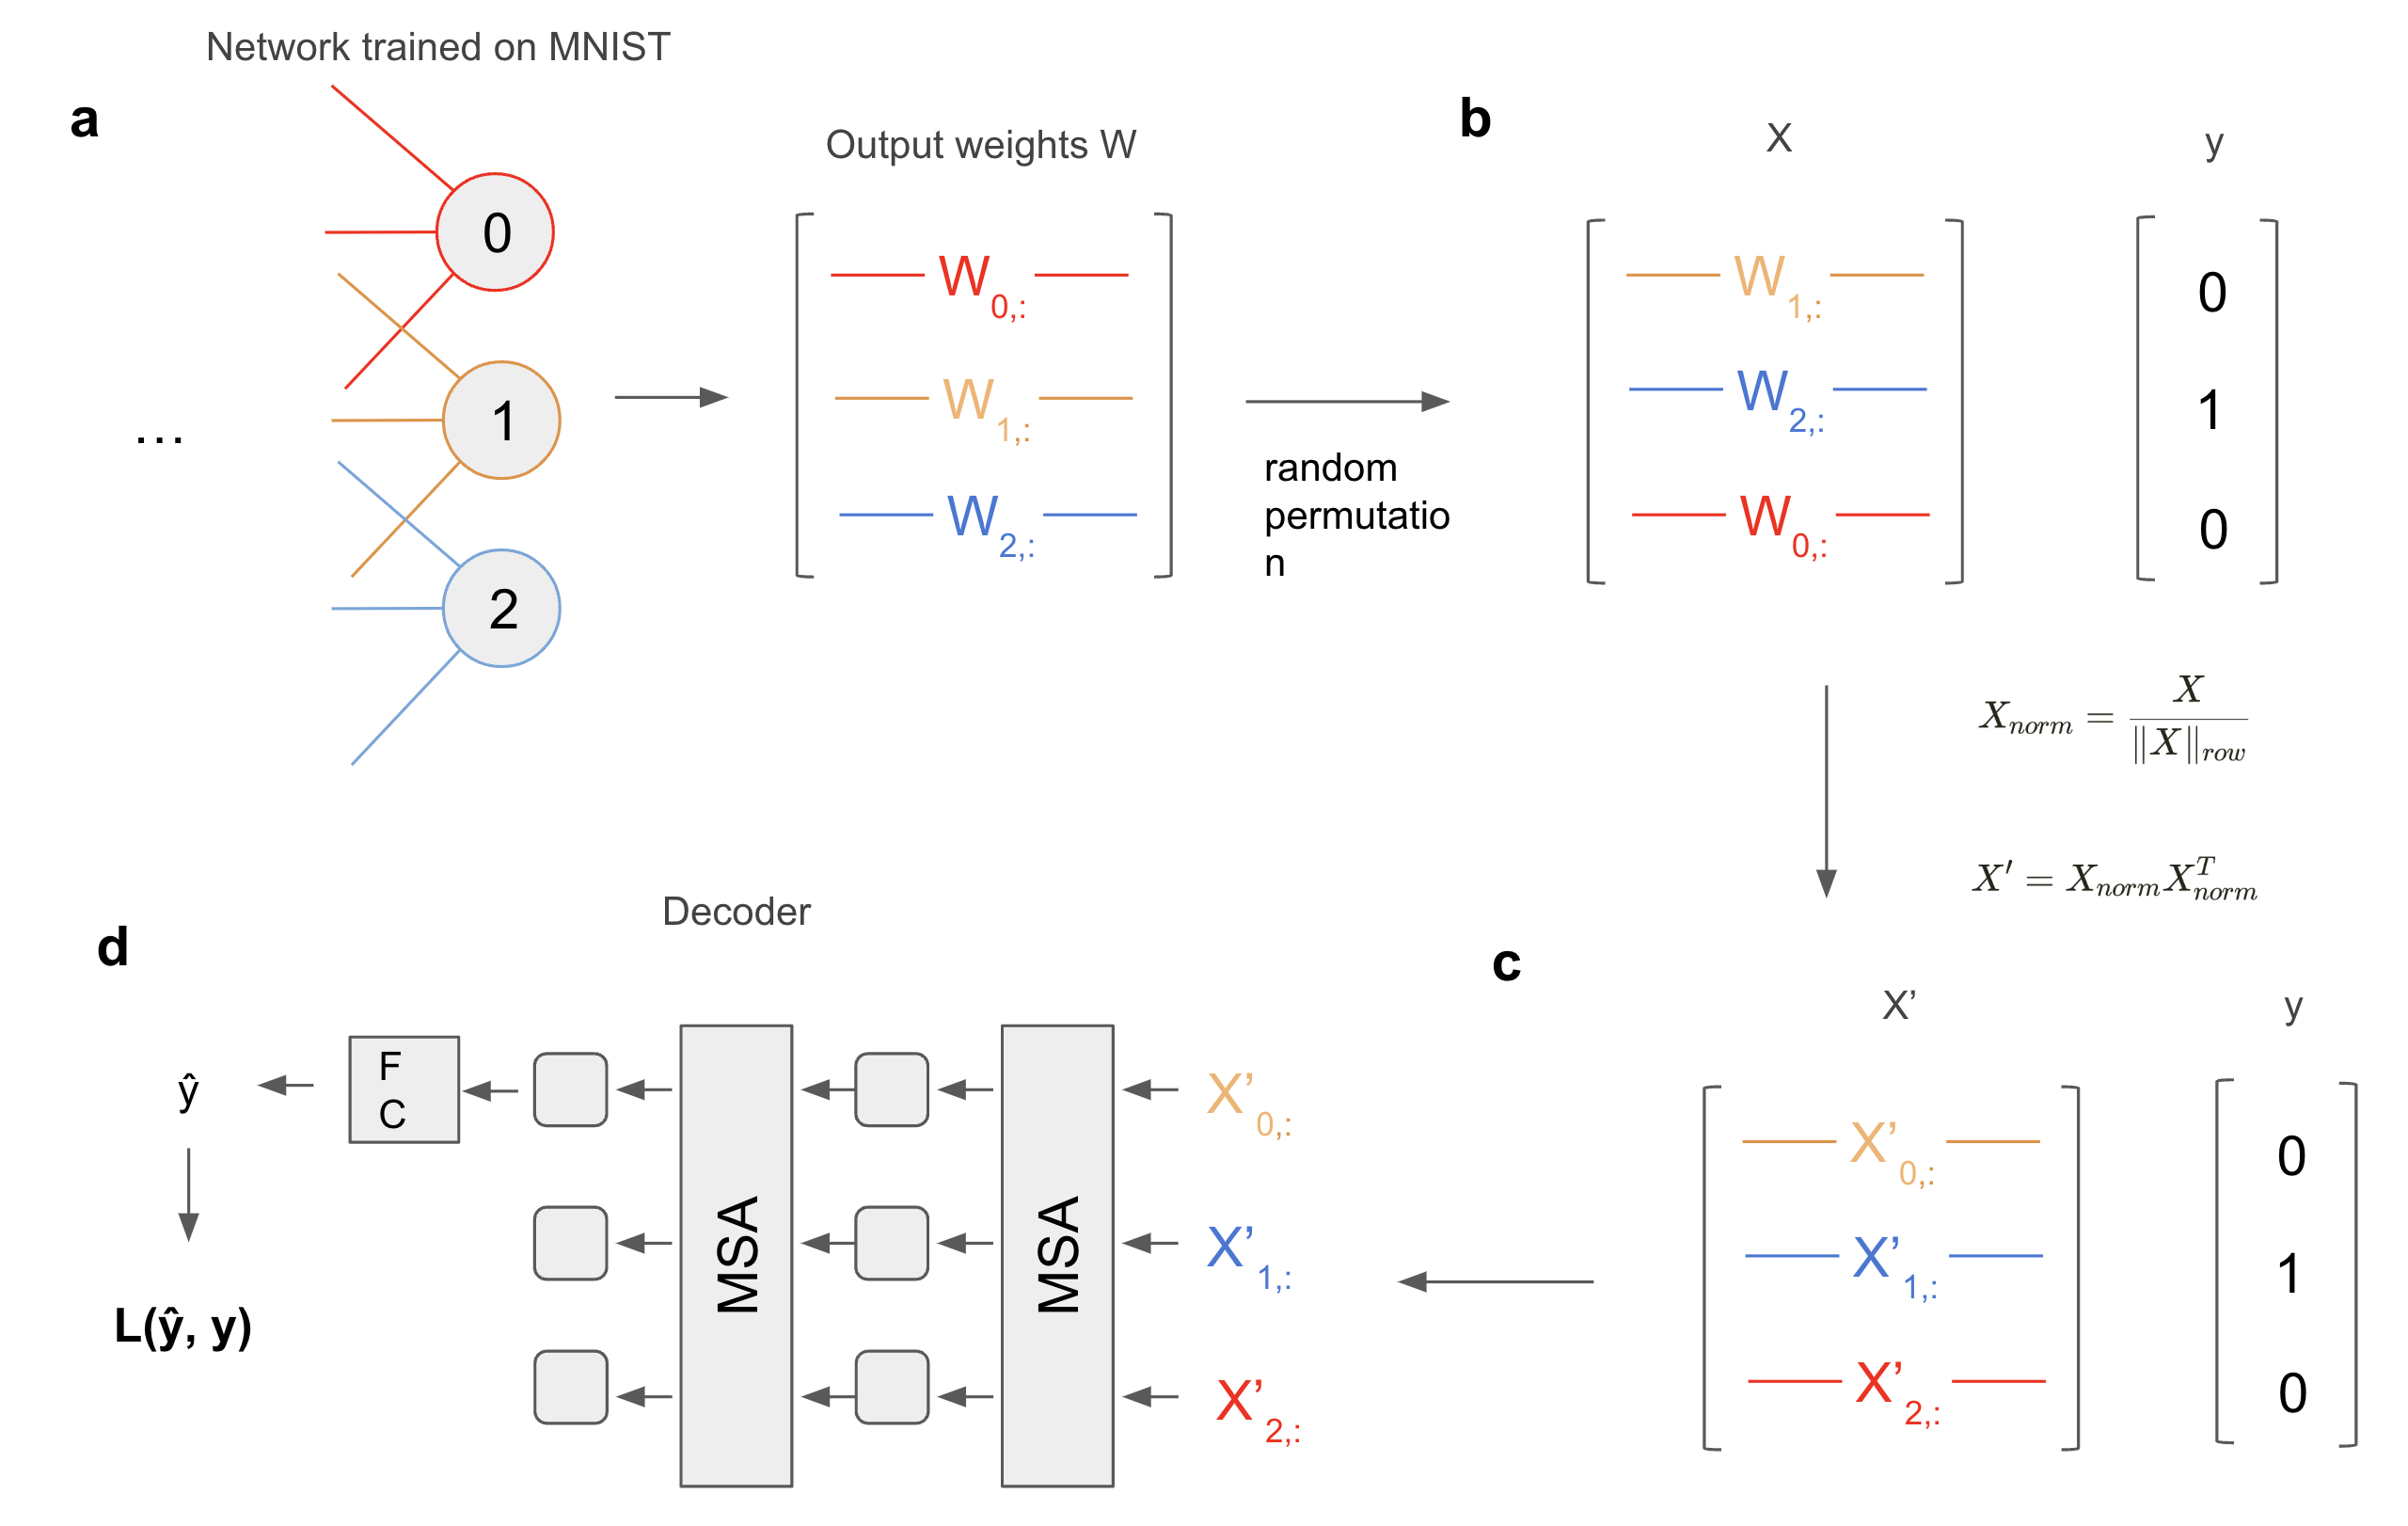
\includegraphics[width=\textwidth]{figures/decoder-architecture-pipeline.png}
\caption{Decoder architecture pipeline: Data processing pipeline from underlying MNIST-trained network to decoder. To simplify the diagrams, we are considering a hypothetical network with only 3 output units. \textbf{(a)} As a basis for our decoding task we consider the output layer of a fully-connected feedforward network trained to classify MNIST using backpropagation. The connectivity matrix contains the incoming weights for each output neuron in its rows. \textbf{(b)} To create a data point for the decoder, we permute the rows of the output layer connectivity matrix such that the class identity of an output neuron cannot be determined based on its position in the matrix. The input weights of the output neuron whose class identity should be predicted is in the first row. \textbf{(c)} To facilitate extraction of relational information between output neurons, we generate matrix $X'$ by first normalizing each row of $X$ and then computing $X' = X_{\text{norm}}X_{\text{norm}}^T$. Each element $(X')_{i,j}$ represents the cosine similarity between the incoming weights of output neuron $i$ and output neuron $j$. \textbf{(d)} The rows of $X'$ are treated as tokens and fed into a multi-head self-attention (MSA) based decoder network. We pass the data through two MSA layers, after which only the representation of the first token is fed into a fully-connected linear layer (FC) which maps to a 10-dimensional space. Finally, during training, the cross-entropy loss (L) is computed between the prediction $\hat{y}$ and the target value $y$.}
\label{fig:decoder-architecture}
\end{figure}

\subsection{Results}

To evaluate whether the output layers of the underlying MNIST networks encode relational information that allows us to identify the class of output neurons, we train our self-attention based decoder for 200 epochs on 8000 datapoints and validate its accuracy on the remaining 2000.

We train the decoder on three different datasets, generated by training fully-connected networks on MNIST in three different training paradigms: no training, normal backpropagation, and backpropagation with dropout. The `no training' paradigm serves as a control. Since the underlying network connectivity is random, there should be no relevant relational structure in the output weights, and hence the decoder accuracy should be equivalent to random guessing (i.e., 0.1). The results are shown in Figure~\ref{fig:decoder-validation-accuracy}.

We can see that the accuracy of predicting output neuron classes based on their connectivity is above chance level (except for the control dataset of untrained networks, which yields chance-level accuracy as expected). Due to the way we designed our dataset, we can be fairly certain that the decoder achieves this purely based on relational information between output neurons.

While training the decoder on the standard MNIST-trained networks (no dropout) yields some correct predictions resulting in a validation accuracy of roughly 25\% at the end of training, the final accuracy jumps to about 75\% as we switch to the dataset that was produced with dropout.

Intuitively we are not surprised that dropout yields higher decoding accuracy, as it encourages neurons to rely on population activity rather than single-neuron pathways \cite{baldi2013}. If output neurons rely on population activity of the last hidden layer, output neurons of similar MNIST digits should also have similar input weights, as they should share more features than output neurons representing dissimilar MNIST digits.

\begin{figure}[htbp]
\centering
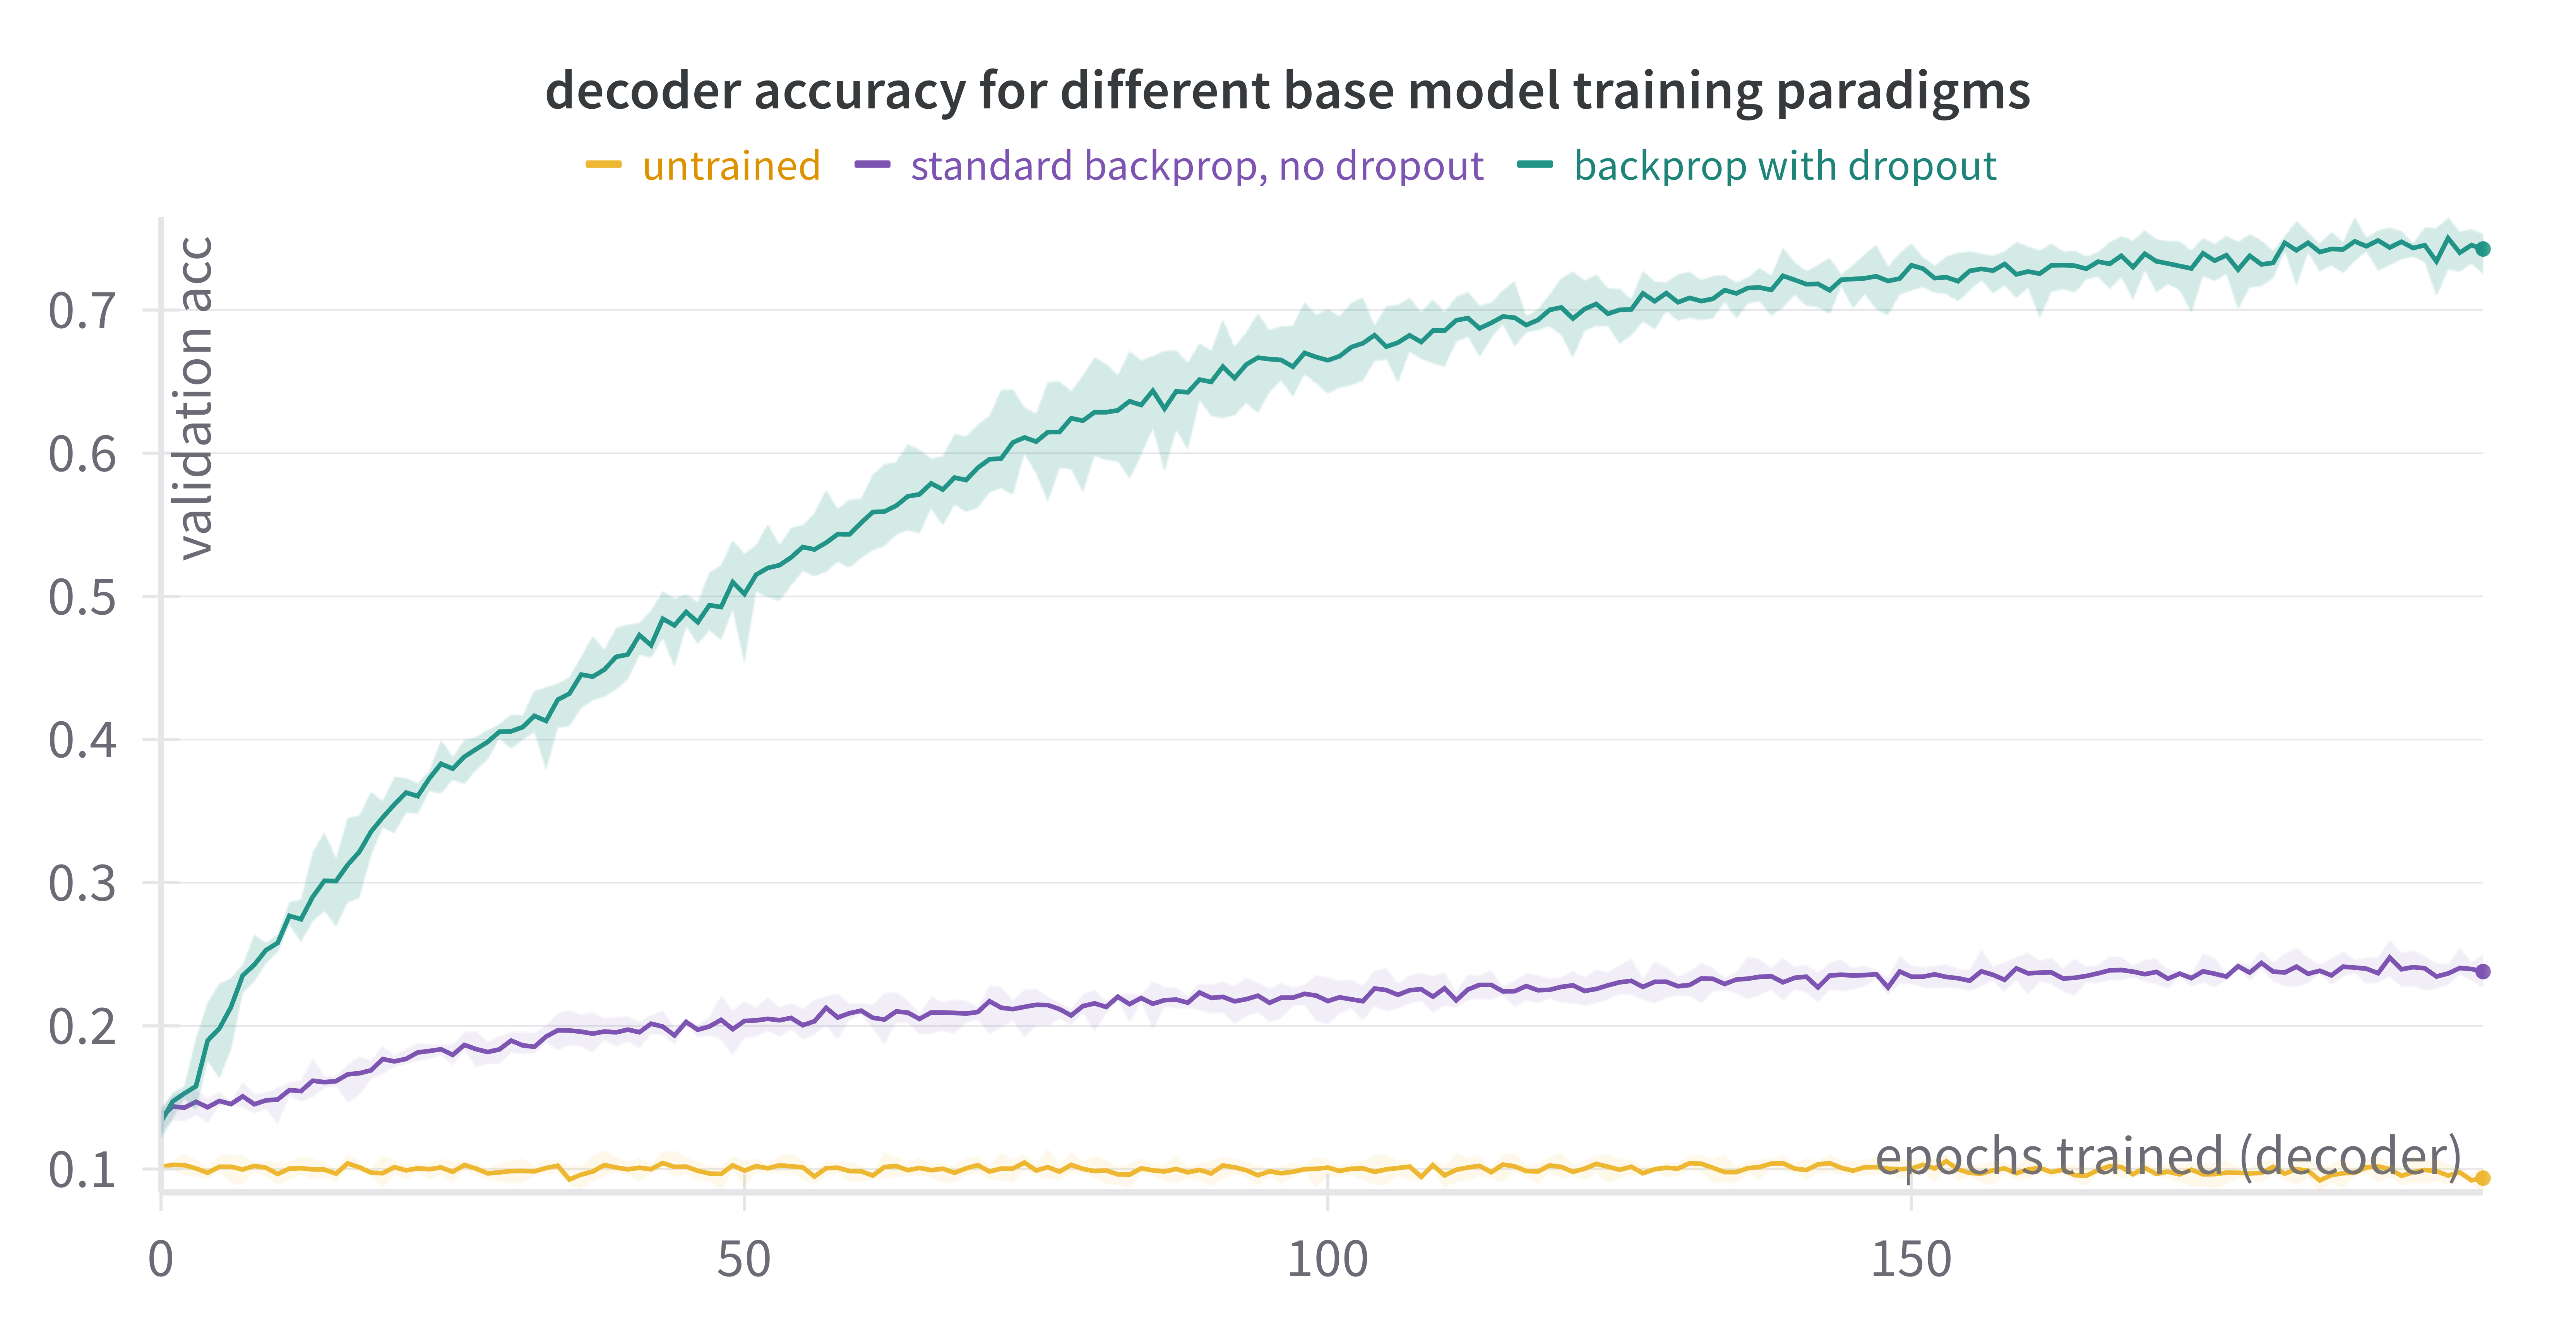
\includegraphics[width=0.8\textwidth]{figures/decoder-validation-accuracy-training-paradigms.png}
\caption{Decoder validation accuracy across training paradigms: Progression of the validation accuracy during 200 epochs of training the decoder to identify output neuron classes based on an unordered set of weight vectors of output neurons. The error margins reflect the standard deviation across 5 random seeds. We used three different training paradigms to generate the underlying MNIST-trained networks used to generate the data for the decoder: no training, normal backpropagation (FullyConnected), and backpropagation with dropout (FullyConnectedDropout). Note that the `untrained' flag in the legend refers to the underlying networks used to generate the training data, not the decoder.}
\label{fig:decoder-validation-accuracy}
\end{figure}

To provide additional context for our results, we show the validation accuracies of the underlying MNIST models themselves (not the decoder) in Figure \ref{fig:mnist-accuracies}. This comparison serves as an important sanity check and further highlights a key insight: despite the dropout-trained networks achieving virtually the same MNIST classification accuracy compared to the standard backpropagation networks, they yield dramatically higher decoder accuracies (75\% vs 25\%). This disparity suggests that dropout fundamentally alters how information is represented within the network, creating more distinct relational structures between output neurons while leaving task performance unchanged.

\begin{figure}[htbp]
\centering
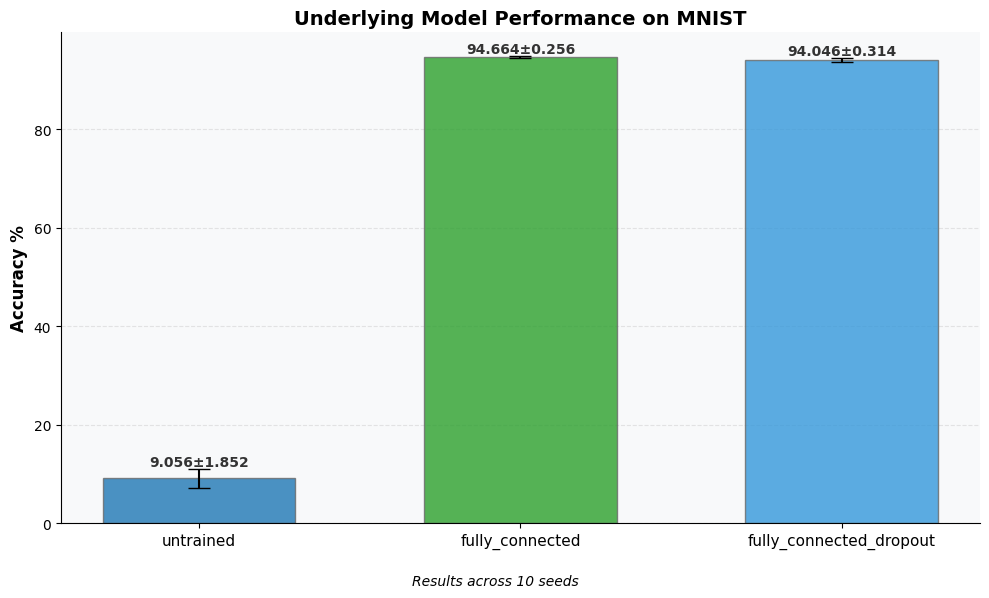
\includegraphics[width=0.8\textwidth]{figures/mnist-model-validation-accuracies.png}
\caption{MNIST model validation accuracies: Validation accuracies of the underlying MNIST models used to generate datasets for the decoder across 10 randomly sampled seeds for each training paradigm.}
\label{fig:mnist-accuracies}
\end{figure}

To pinpoint how much of the decoder's success comes from the whole relational geometry of the output layer, we reran the experiment but supplied the decoder with only the first row of X', the cosine-similarity vector of the target neuron with all other neurons in the output layer, while masking out all pairwise similarities that do not involve the target neuron.

\begin{figure}[htbp]
\centering
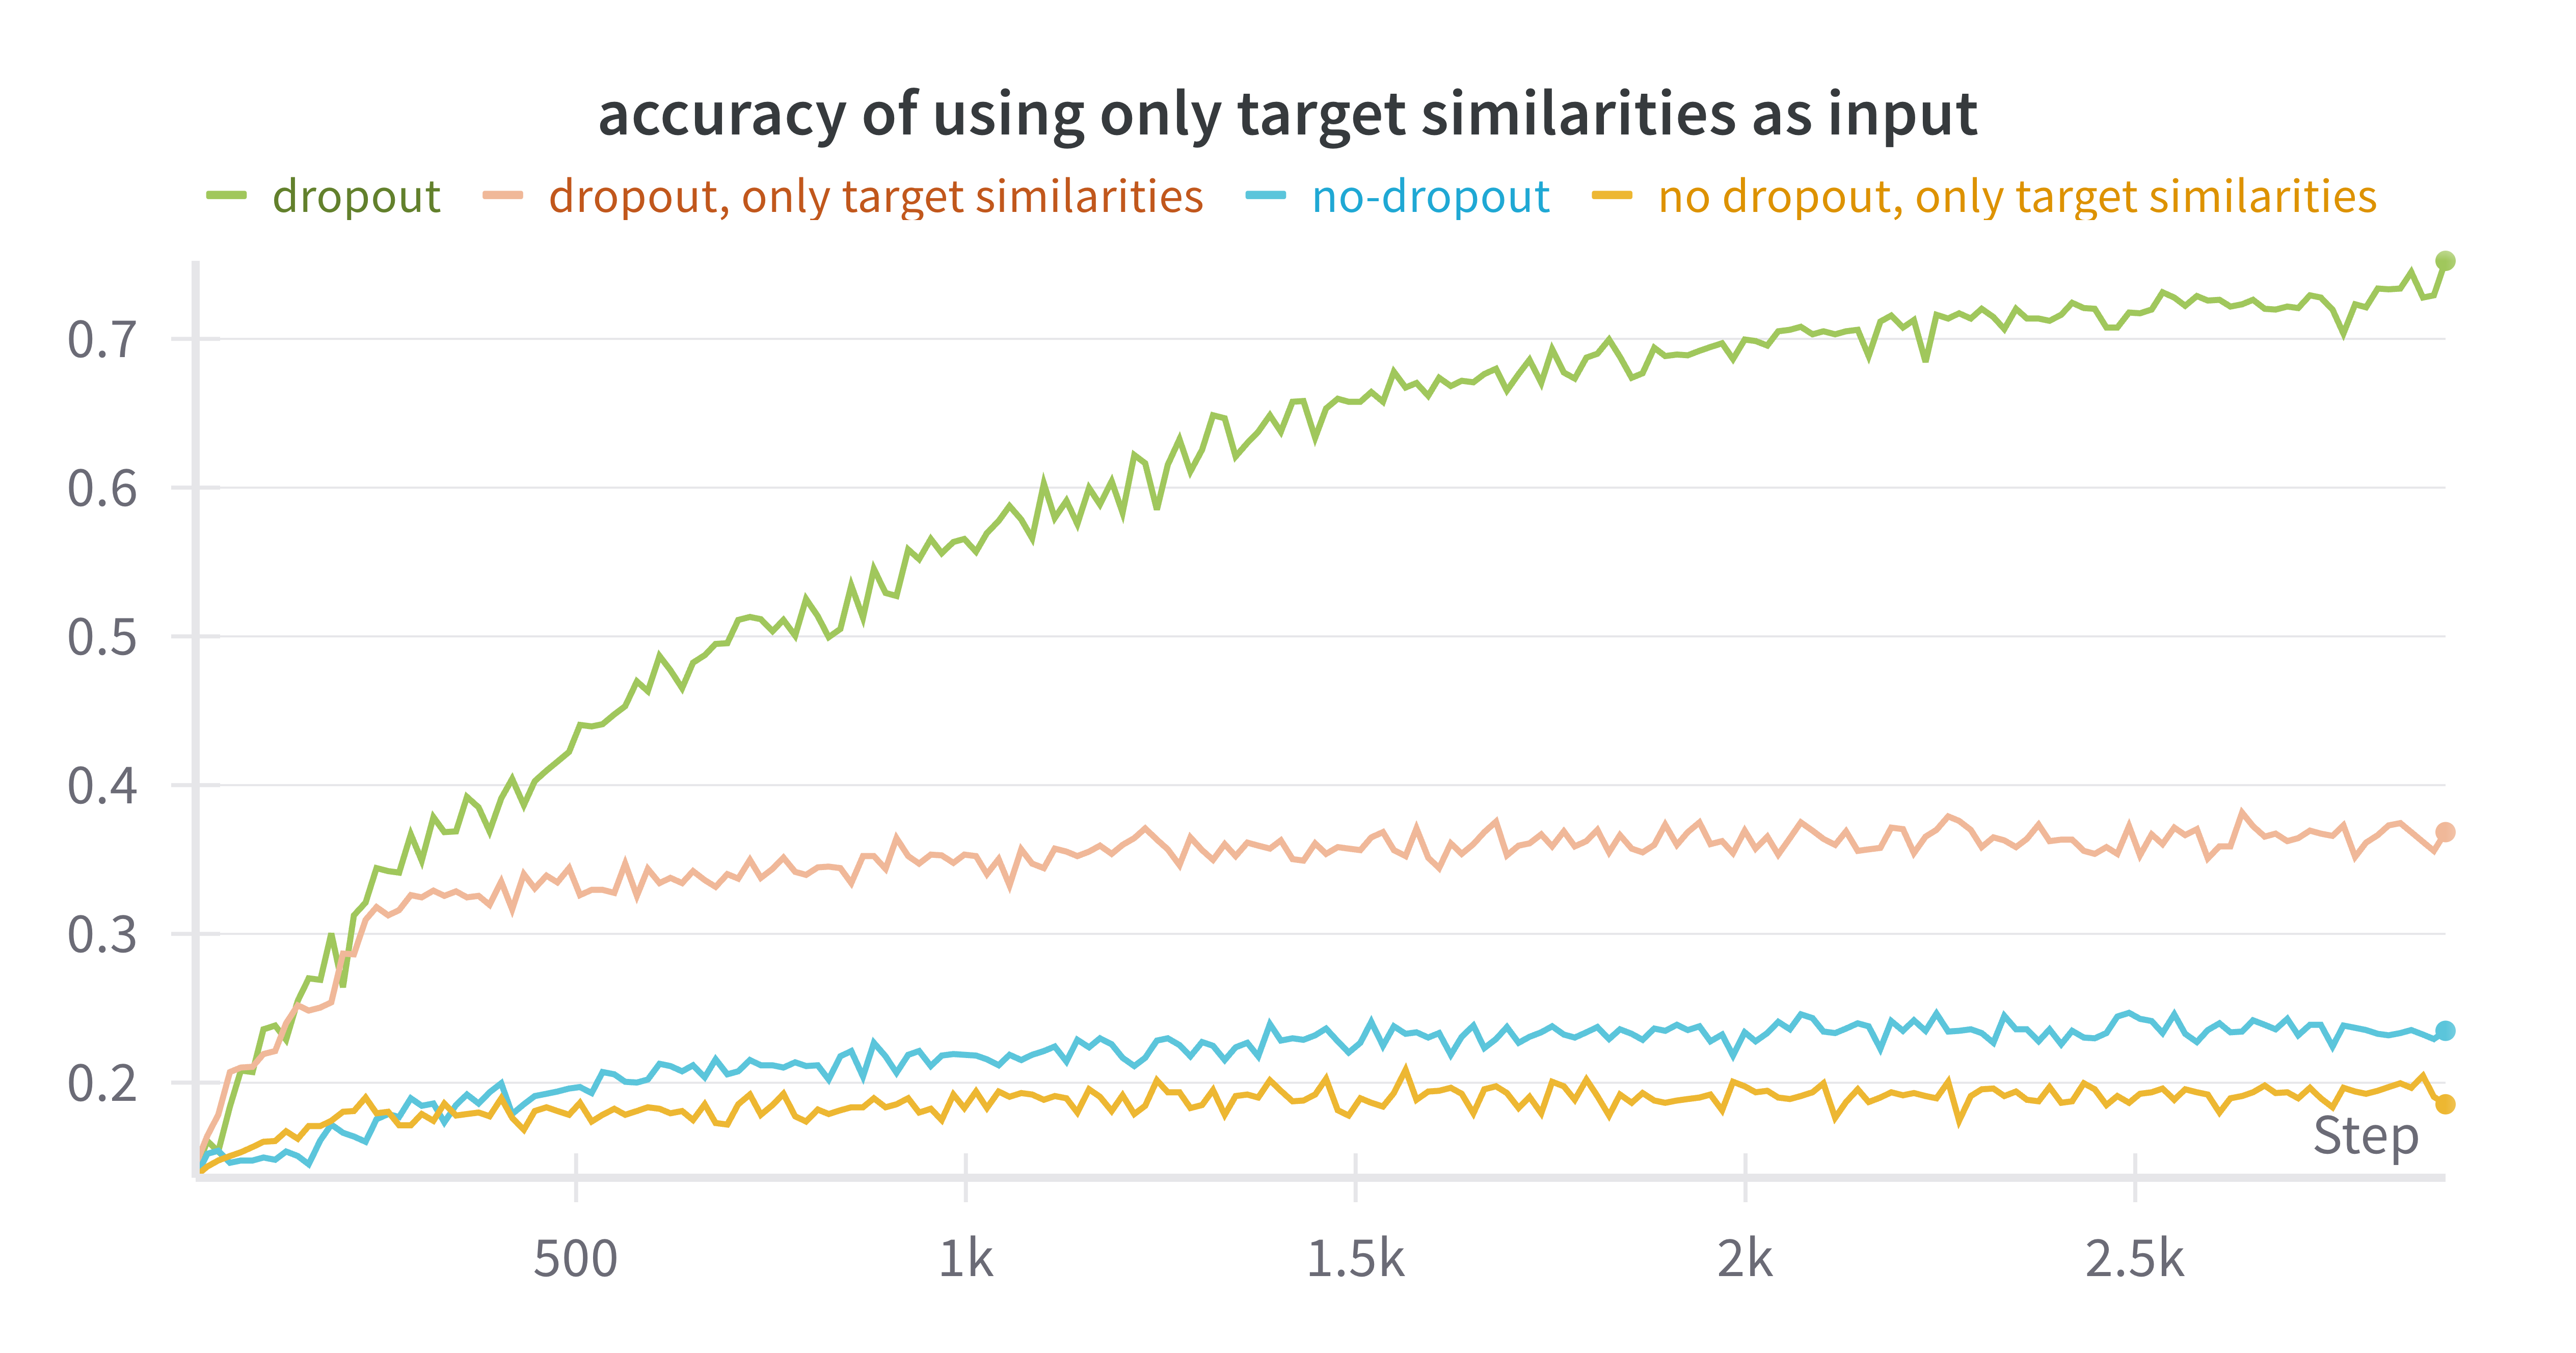
\includegraphics[width=0.8\textwidth]{figures/target-similarity-only-output-neurons.png}
\caption{Target similarity only for output neurons: Accuracy plummets when contextual relational structure is removed, showing that a single neuron's local neighborhood is insufficient to accurately determine its class identity.}
\label{fig:target-similarity-output}
\end{figure}

Figure \ref{fig:target-similarity-output} shows that accuracy plummets when that contextual structure is removed (for both vanilla backprop and dropout). This shows that a single neuron's local neighborhood is insufficient to accurately determine its class identity; the decoder takes into account how the rest of the output population is organized to disambiguate which digit the target neuron represents.

To gauge how architecture-invariant our decoder really is, we check whether it can maintain high classification accuracy when the base network layout changes. Figure \ref{fig:architecture-transfer} summarizes the result for an unseen target architecture: a decoder trained only on [50, 50] already transfers above chance, while a decoder trained on networks whose layer width is randomly sampled between 25 and 100 climbs almost to the self-transfer performance, demonstrating near-architecture-independent generalization.

\begin{figure}[htbp]
\centering
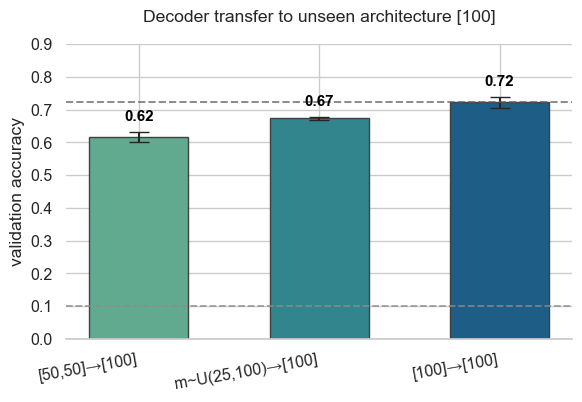
\includegraphics[width=0.8\textwidth]{figures/architecture-transfer-evaluation.png}
\caption{Architecture Transfer Evaluation: Cross-architecture transfer performance showing how well decoders generalize across different network architectures.}
\label{fig:architecture-transfer}
\end{figure}

To investigate how relational structure complexity affects decoding accuracy, we conducted an ablation study by systematically reducing the number of output neurons available to the decoder. Our results shown in Figure \ref{fig:ablation-study} confirm that asymmetric relational structures between output neurons are essential for the decoder to function: The 2-neuron case performs exactly at random chance level (50\%, or 1.0x), since asymmetric relations cannot exist between only two points. While the 5-neuron condition achieves the highest absolute validation accuracy (79.1\%), performance relative to random guessing increases consistently with neuron count, with the 10-neuron model performing 7.36x better than random (73.6\%). This suggests that as the decoder gains access to more relational structure among output neurons, it becomes increasingly capable of decoding that structure, implying that decoder accuracy should continue to improve with more complex input distributions as the ambiguity of underlying representations decreases.

\begin{figure}[htbp]
\centering
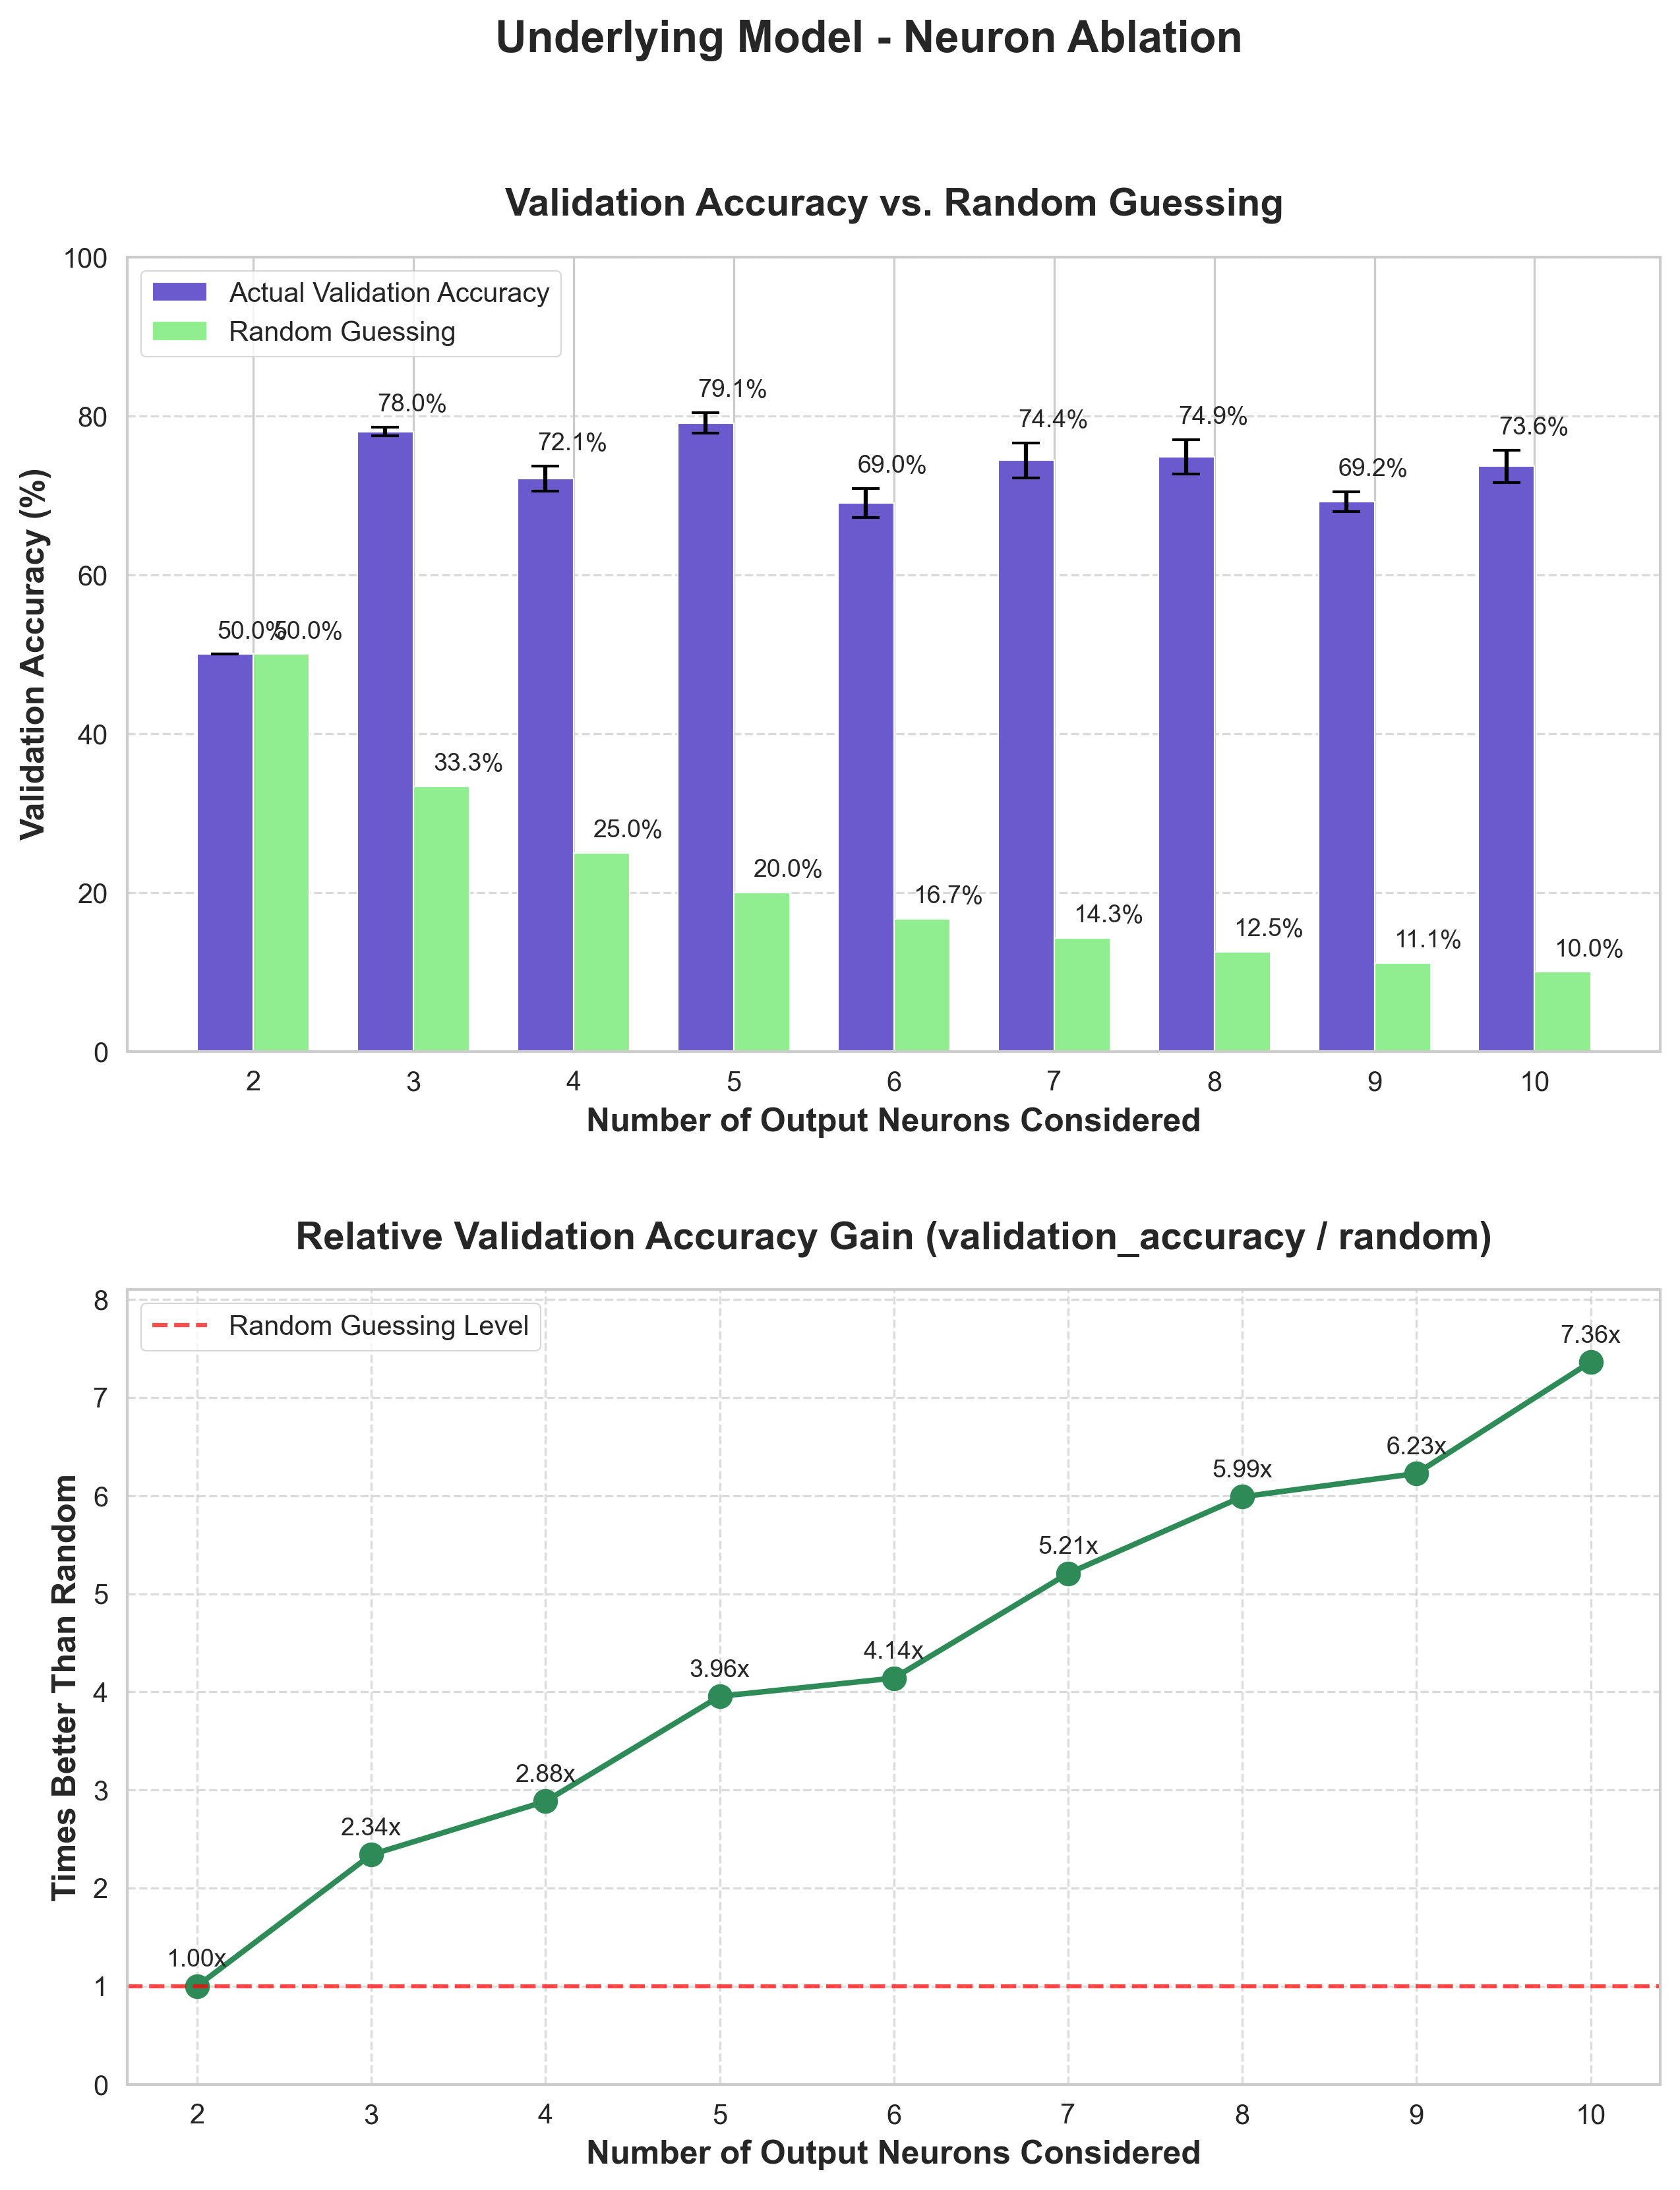
\includegraphics[width=0.8\textwidth]{figures/ablation-study-neuron-count-performance.png}
\caption{Ablation study showing neuron count performance: Ablation study examining the impact of neuron count on neural network performance. The top panel compares validation accuracy (purple) to the random guessing baseline (green) for networks with 2-10 output neurons. Error bars represent standard deviation across 5 random seeds for each condition. The bottom panel shows the relative performance gain compared to random guessing. The 2-neuron case achieves only random-level performance (1.0x), validating the hypothesis that asymmetric relational structures in the output layer are necessary for the decoder to function. Performance relative to random chance increases with neuron count, with the 10-neuron model achieving 7.36x better than random performance.}
\label{fig:ablation-study}
\end{figure}

\subsection{Geometric Matching Approach}

Having established that learned decoders can successfully extract relational structure from neural network connectivity, we investigated whether the geometric structure itself is sufficiently distinctive and consistent across networks to enable direct matching without requiring a trained decoder.

This method constructs a reference Gram matrix by averaging the cosine similarity matrices from several reference networks trained on MNIST. For each validation network, we then evaluate all possible permutations of its output neurons to find which ordering produces a Gram matrix closest to the reference geometry using Frobenius distance. If relational representations are truly unambiguous and consistent across network instances, the correct class ordering should yield the best match to the reference geometry.

\begin{center}
\begin{tabular}{lcc}
\toprule
Model & Accuracy & Std Dev \\
\midrule
untrained & 0.100 & 0.155 \\
no\_dropout & 0.383 & 0.441 \\
dropout & 1.000 & 0.000 \\
\bottomrule
\end{tabular}
\end{center}

\textit{Gram matrix decoding accuracies across training paradigms using 5 reference networks and 10 validation networks.}


The results validate this hypothesis. This geometric approach achieves remarkably higher accuracies than the self-attention decoder, reaching perfect 100\% accuracy for dropout-trained networks while requiring significantly fewer reference networks. The untrained networks perform at chance level as expected, while standard backpropagation networks achieve 38.3\% accuracy.

The dropout condition achieves perfect decoding with zero variance, showing that dropout creates consistent and distinctive relational geometries between output neurons across different network instances.

Similar to our earlier ablation study with the self-attention decoder, we investigated how the number of output neurons affects the Gram matrix matching approach. Results are shown in \ref{fig:permutation-distances}

\begin{figure}[htbp]
\centering
\begin{subfigure}[b]{0.45\textwidth}
\centering
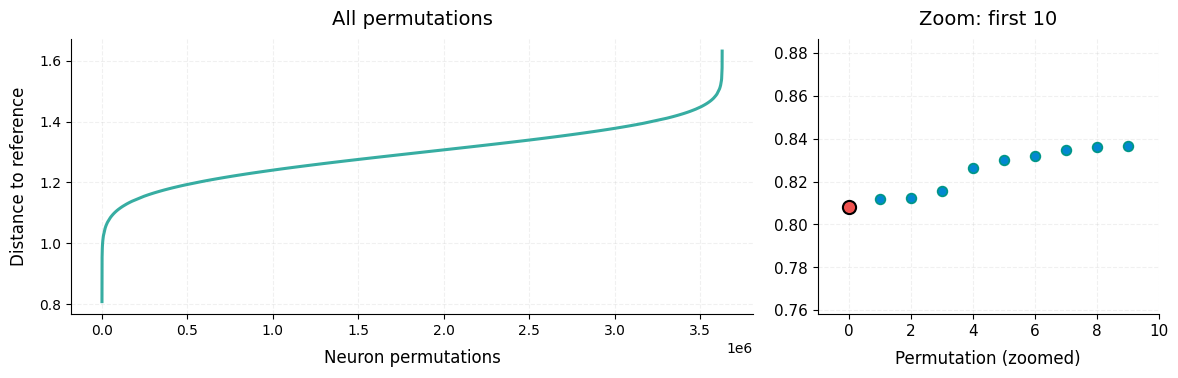
\includegraphics[width=\textwidth]{figures/perm_distances_no_dropout.png}
\caption{No dropout networks}
\label{fig:perm-no-dropout}
\end{subfigure}
\hfill
\begin{subfigure}[b]{0.45\textwidth}
\centering
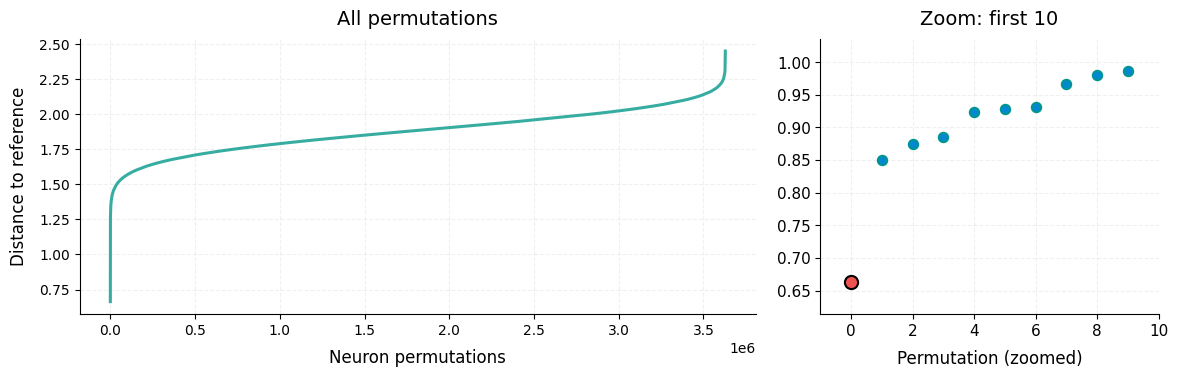
\includegraphics[width=\textwidth]{figures/perm_distances_dropout.png}
\caption{Dropout networks}
\label{fig:perm-dropout}
\end{subfigure}
\caption{Permutation distance distributions: \textbf{(a)} For networks trained without dropout, the true permutation (red dot) shows only a small margin over incorrect permutations. \textbf{(b)} For networks trained with dropout, the true permutation shows a substantial gap from all incorrect alternatives.}
\label{fig:permutation-distances}
\end{figure}

\begin{figure}[htbp]
\centering
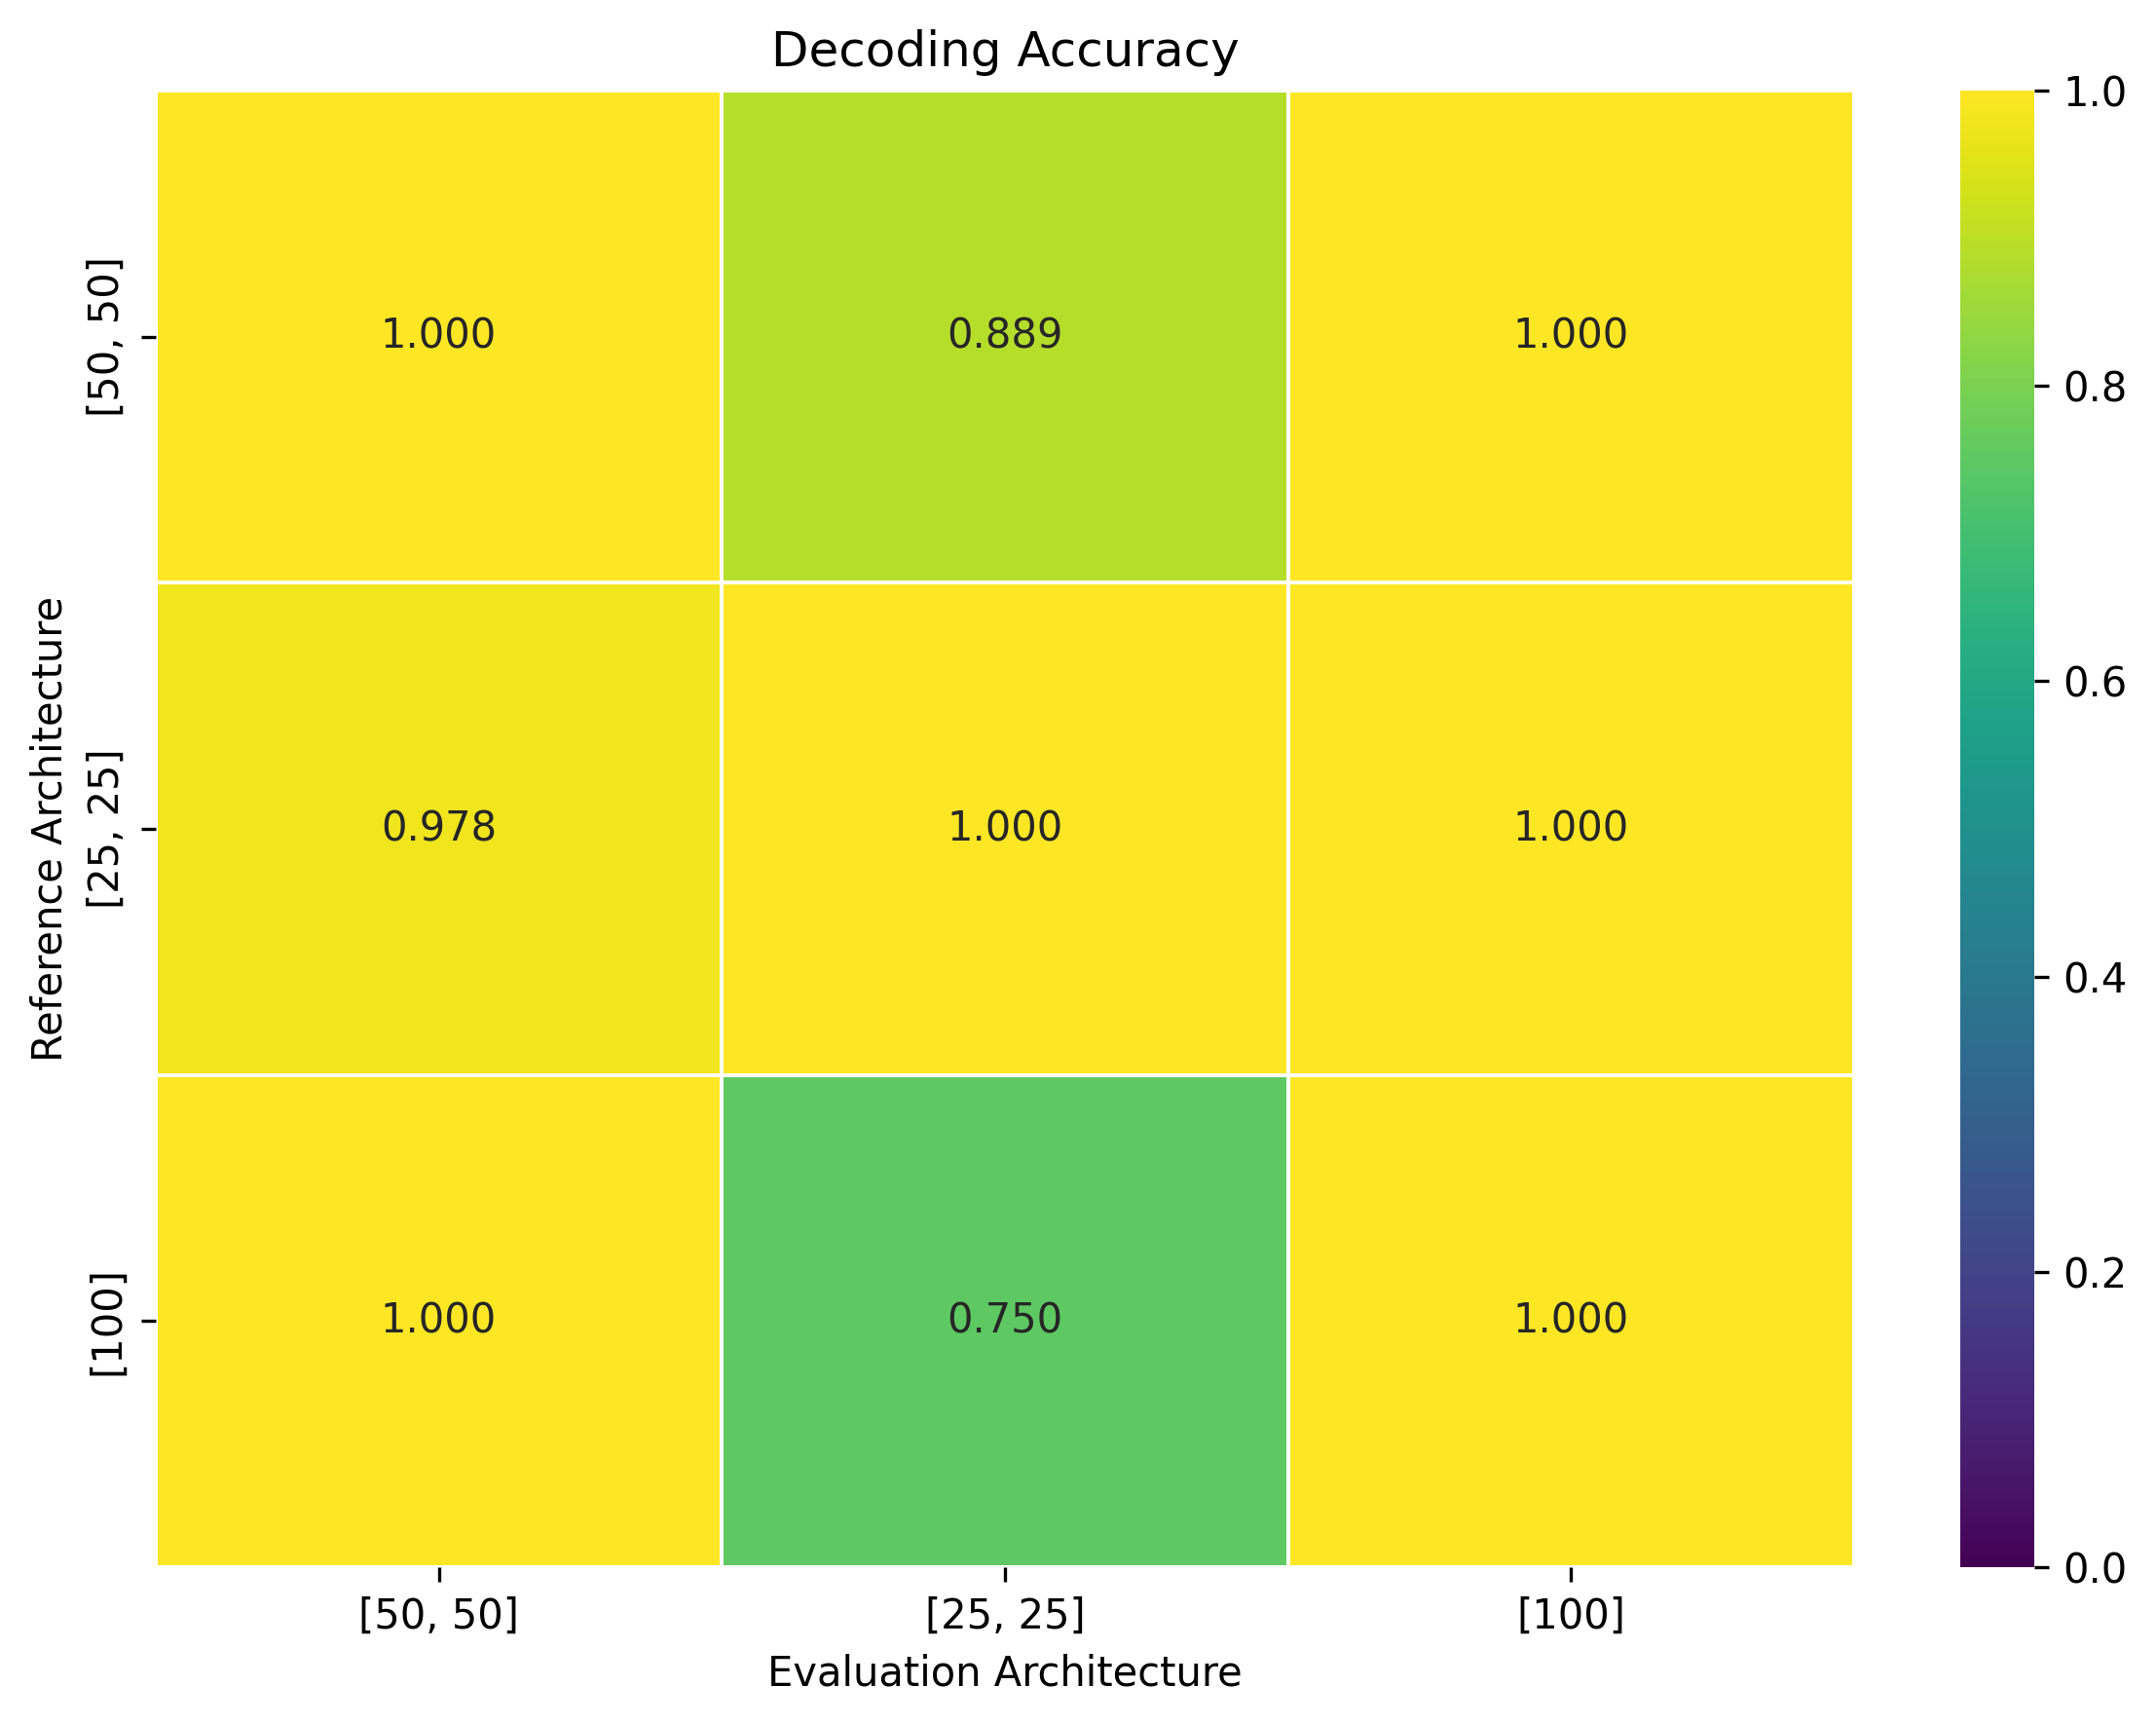
\includegraphics[width=0.8\textwidth]{figures/cross_architecture_heatmap_accuracy.png}
\caption{Cross-architecture transfer evaluation: Decoding accuracy when transferring between different network architectures. Each cell represents accuracy when using reference networks of one architecture (y-axis) to decode test networks of another architecture (x-axis). The strong diagonal performance demonstrates architecture-invariant relational geometric structure.}
\label{fig:cross-architecture}
\end{figure}

\subsection{Hyperparameters}

In the following we list all hyperparameters that were chosen for the underlying networks to generate the dataset (Table~\ref{tab:mnist-params}), and for the self-attention based decoder (Table~\ref{tab:decoder-params}). Note that none of these hyperparameters were optimized using gridsearch or similar schemes, most of them were chosen quite arbitrarily, since this is only supposed to be a proof of concept.

\begin{table}[htbp]
\centering
\begin{tabular}{lr}
\toprule
Name & Value \\
\midrule
learning rate & 0.001 \\
batch size & 256 \\
epochs (except for the non-train paradigm) & 2 \\
hidden dimensionalities & 50, 50 \\
dropout rate (only for the dropout paradigm) & 0.2 \\
\bottomrule
\end{tabular}
\caption{Hyperparameters for underlying, MNIST-trained networks used to generate the training and validation data for the decoder. Note that the number of epochs in the 'untrained' paradigm was set to 0, and the dropout rate only applies to the 'dropout' paradigm.}
\label{tab:mnist-params}
\end{table}

\begin{table}[htbp]
\centering
\begin{tabular}{lr}
\toprule
Name & Value \\
\midrule
learning rate & 0.001 \\
batch size & 64 \\
epochs & 200 \\
hidden dimensionality & 128 \\
number of attention heads per MSA layer & 4 \\
number of MSA layers (encoder) & 2 \\
number of fully connected layers & 1 \\
\bottomrule
\end{tabular}
\caption{Hyperparameters for decoder. MSA is short for multi-head self-attention.}
\label{tab:decoder-params}
\end{table}

\subsection{Dataset Identity from Final-Layer Weights}

Using the same self-attention decoder and random output-neuron permutations, we classify whether a network was trained on MNIST or Fashion-MNIST from the final-layer weights alone. Performance is near-perfect for Dropout models (0.998 ± 0.001 STD) and clearly above chance for No Dropout (0.843 ± 0.008 STD). This indicates that the relational geometry of the output weights carries a dataset-specific signature, amplified by dropout.

\begin{figure}[htbp]
\centering
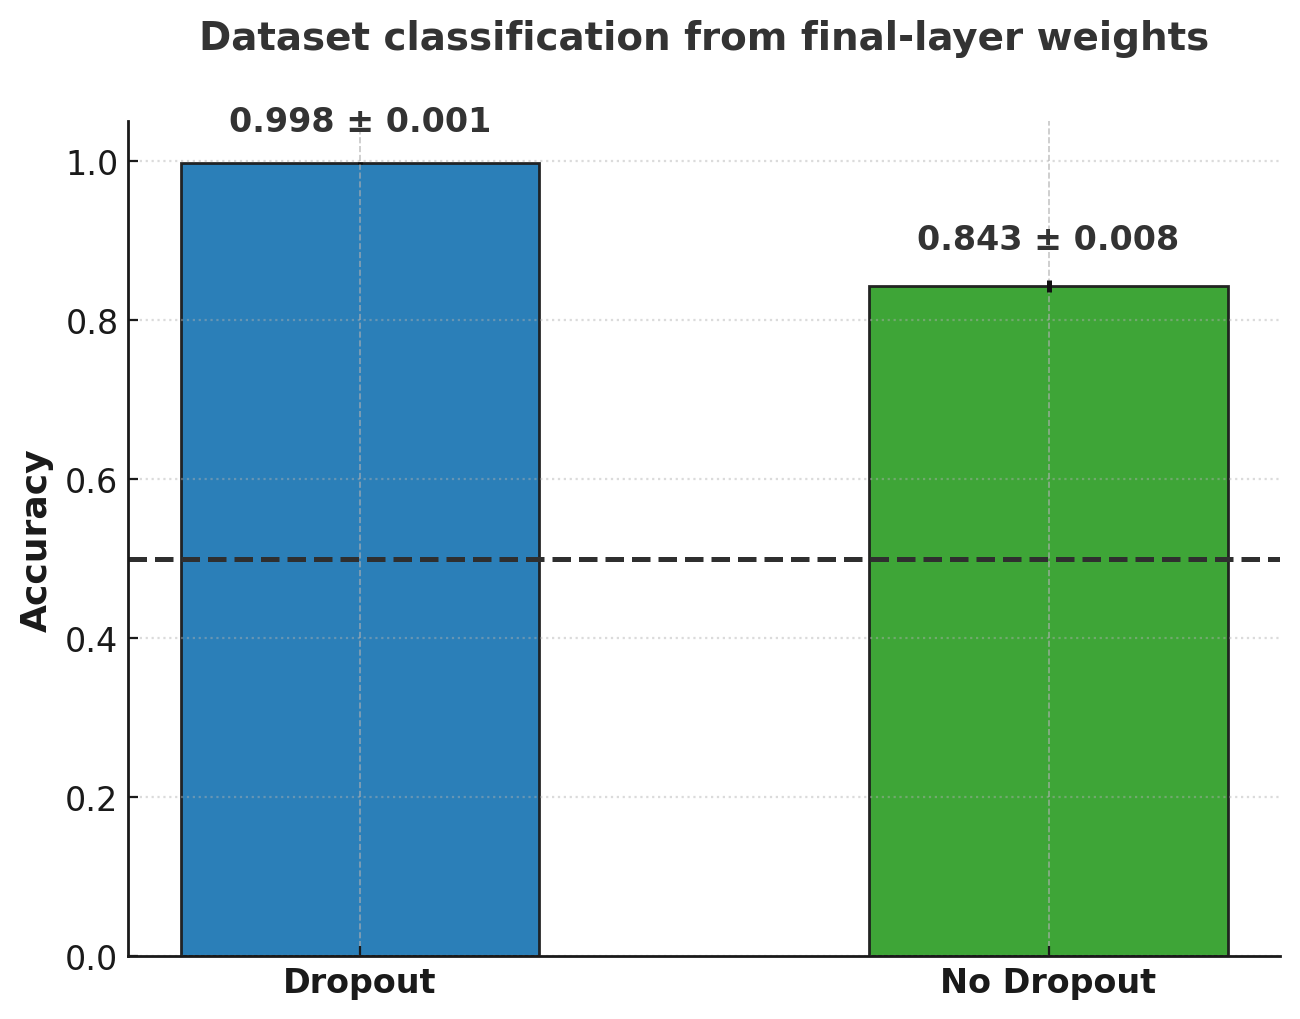
\includegraphics[width=0.7\textwidth]{figures/dataset-classification-accuracy.png}
\caption{Dataset classification from final-layer weights showing validation accuracy for distinguishing MNIST from Fashion-MNIST networks based solely on output layer connectivity patterns.}
\label{fig:dataset-classification}
\end{figure}

\subsection{3D Embedding of Reference Gram Matrix}

To further visualize the relational structure that enables perfect decoding in dropout networks, we performed eigendecomposition on the reference Gram matrix and embedded the 10 neuron positions into 3D space using the top 3 eigenvectors, scaled by their corresponding eigenvalues. The connecting edges highlight nearest-neighbor relationships, revealing the geometric structure underlying the perfect classification performance.

\begin{figure}[htbp]
\centering
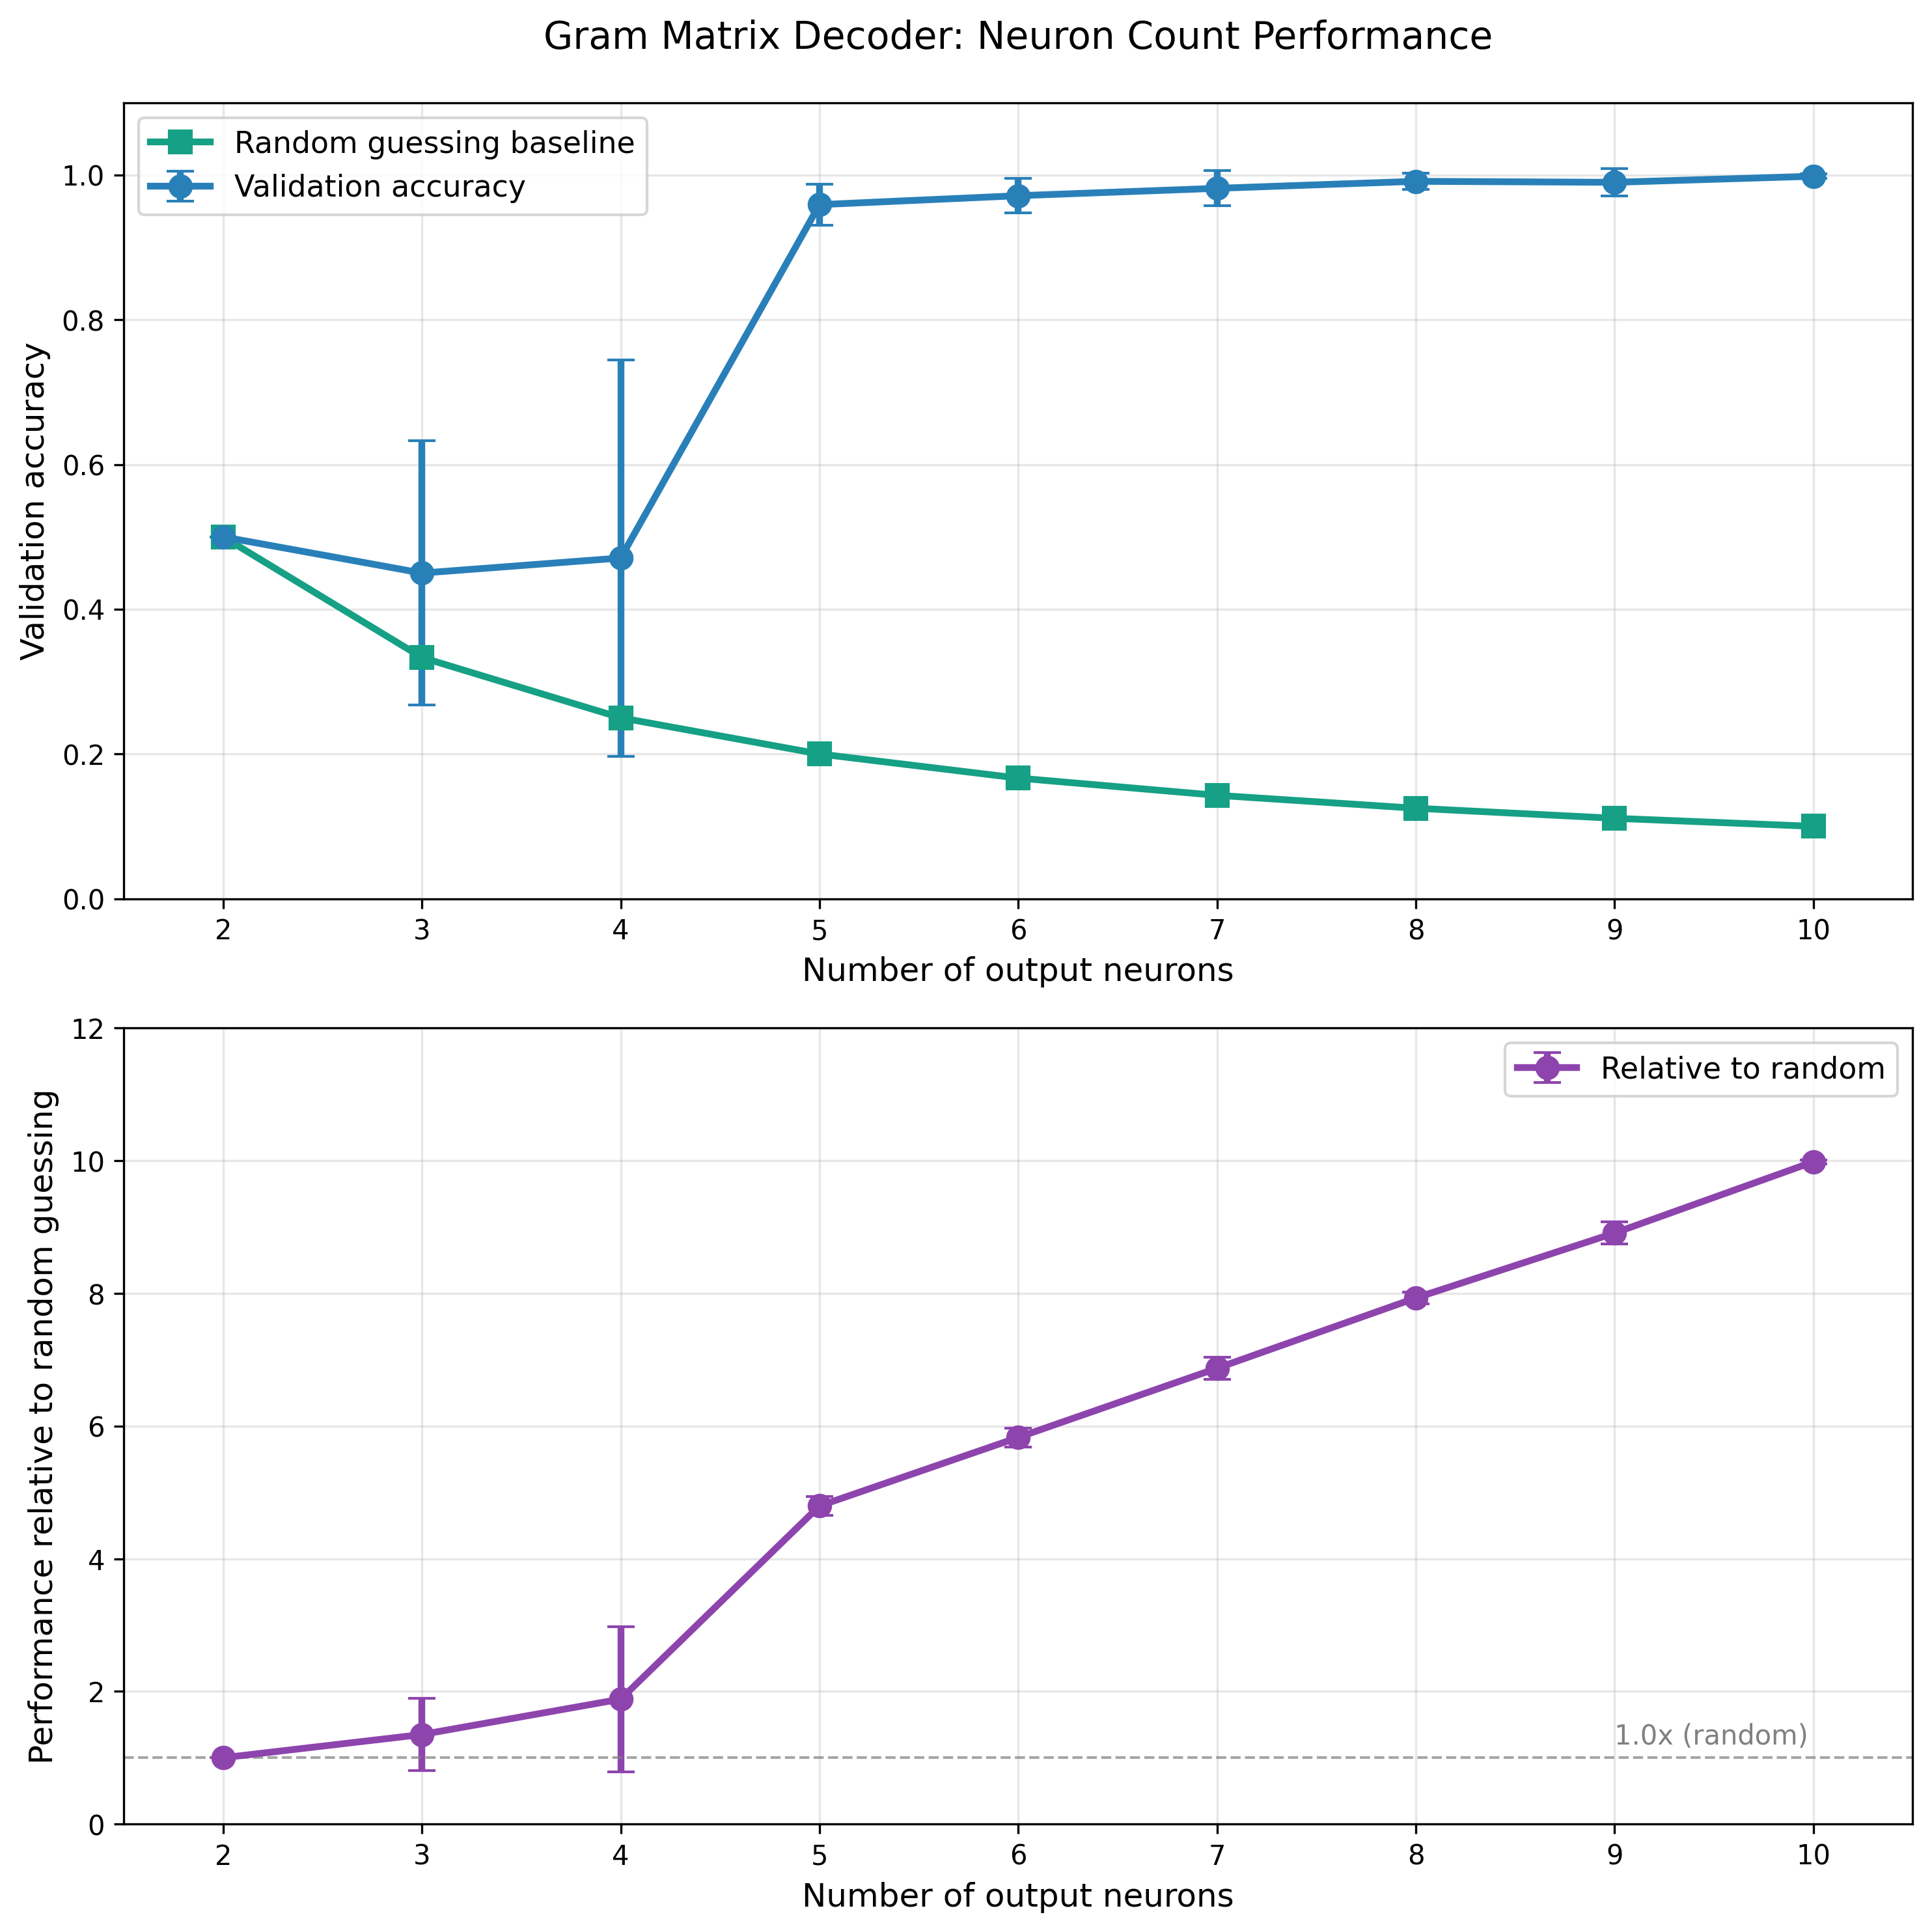
\includegraphics[width=0.8\textwidth]{figures/gram_neuron_ablation_plot.png}
\caption{Gram matrix decoding performance vs. number of neurons: Ablation study showing how Gram matrix matching accuracy varies with the number of output neurons available for decoding.}
\label{fig:gram-ablation}
\end{figure}

\section{Exhibit 2: Input Neuron Representation}

\subsection{Idea}

In the previous exhibit we showed strong evidence for abstract digits being represented in an unambiguous relational structure that can be leveraged to identify class identity from randomly shuffled output neurons. However, because of the abstract nature of class identity, the link to phenomenal consciousness might be unintuitive. This is especially true if one thinks of phenomenal consciousness as applying more to the sensory than the abstract.

So, let's turn the tables and look at input neurons! This links back to the introductory example of the 2D grid in relational structures as unambiguous representations. In this case, we know that the input neurons represent a grid of input pixels, as that's how they are used in a forward pass. But is there a sense in which this information is intrinsic to the network connectivity?

To frame it as a decoding problem: given the first layer weight matrix with permuted columns (where rows correspond to the neurons of the first hidden layer and columns to input neurons), can we infer positional information about input neurons? While the strictest version of this task would be to identify the exact coordinates of an input neuron, we can also consider weaker versions, such as identifying only one coordinate, or the proximity to the center.

Please note that only considering one layer for this decoding task serves several purposes:

\begin{enumerate}
\item It simplifies our experiment and leaves fewer degrees of freedom for operationalization.
\item It precludes solutions to the decoding task that involve passing sample inputs through the whole network, e.g., for testing to what extent input neurons affect output neurons for different inputs.
\end{enumerate}

Moreover, since we will apply the same cosine similarity preprocessing step as in the previous experiment, we can also prevent other `trivial' solution methods such as inferring positional information from the norm of the outgoing weights of an input neuron.

Preliminary visualizations using UMAP on the cosine similarity matrix between input neurons of a trained network (no dropout) already suggest that some positional information is present and decodable relationally.

\subsection{Machine Learning Setup}

To operationalize this idea, we cast it as a supervised learning problem. We define a function $f(i, j)$ that extracts some form of positional information from an input neuron's location $(i, j)$ in the 28×28 grid. The decoder's task is not to learn the function $f$ itself, but to predict the value of $f(i, j)$ \textbf{given only the relational representation} of that neuron relative to all other neurons. In other words, the decoder must infer $f(i, j)$ \textbf{without knowing the values of $i$ or $j$}, purely from the context provided by connectivity structure.

Example functions $f(i, j)$ include:

\begin{itemize}
\item $f(i, j) = (i / 27, j / 27)$ for normalized 2D position.
\item $f(i, j) = i / 27$ for normalized horizontal position.
\item $f(i, j) = j / 27$ for normalized vertical position.
\item $f(i, j) = \sqrt{(i - 13.5)^2 + (j - 13.5)^2}$ for distance from center.
\end{itemize}

This formulation lets us probe different levels of representational structure and ambiguity.

We again use a Set Transformer architecture that is invariant to permutations of the input columns (beyond the first), ensuring that the decoder can only rely on relational information for solving the task. The first column is treated specially because the decoder is trained to predict the positional information of the neuron occupying that column, based on its similarity to all other input neurons.

Note that this contrasts with Exhibit 1, where the decoder predicted output neuron class based on incoming weight \textbf{rows}; here, we operate on \textbf{columns} representing outgoing weights of input neurons.

\subsection{Dataset}

To create training examples, we generate multiple neural networks with the same architecture but different initialization seeds. For each network, we extract the input weight matrix $W$ of shape (784, H), where 784 corresponds to input neurons (pixels), and H is the number of hidden units in the first layer.

To build one training example:

\begin{itemize}
\item We permute the columns of $W$, destroying any trivial positional information.
\item We select one of the columns (i.e., one input neuron) and place it in the first position.
\item The input $X$ to the decoder is then the full permuted weight matrix.
\item The label $y$ is $f(i, j)$ for the input neuron that ended up in the first column.
\end{itemize}

Crucially, the decoder is never given access to the coordinates $(i, j)$ directly—it only sees the connectivity patterns between neurons (encoded in the similarity matrix), and must infer positional information from those alone.

\subsection{Preprocessing}

To make the decoder task explicitly relational, we compute a cosine similarity matrix $X'$ from the \textbf{column vectors} of $W$. This differs from Exhibit 1, where similarities were computed between row vectors (i.e., incoming weights to output neurons). Here, each column represents the outgoing weights of an input neuron into the hidden layer, and their pairwise similarities define a relational structure over input neurons:

\begin{align}
X_{\text{norm}} &= \frac{X}{\|X\|_{\text{col}}} \\
X' &= X_{\text{norm}}^T X_{\text{norm}}
\end{align}

We feed the similarity matrix $X'$ to a Set Transformer-based decoder. This preprocessing emphasizes relational structure by encoding how similar each input neuron is to every other in terms of their effect on the next layer.

\begin{figure}[htbp]
\centering
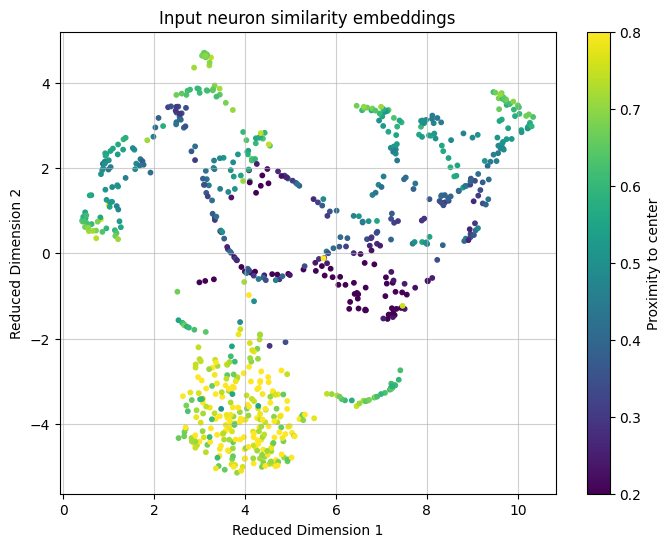
\includegraphics[width=0.7\textwidth]{figures/umap-input-neuron-similarity.png}
\caption{UMAP visualization of input neuron cosine similarity vectors, suggesting that positional information is present and decodable relationally in trained networks.}
\label{fig:umap-input}
\end{figure}

\subsection{Results}

First, we can establish that this task is also solvable, suggesting that relational information encoded in the input neuron outgoing weights is sufficient to determine distance from the center of the pixel they represent (except for the untrained control networks, which serve as a sanity check for our experimental setup).

The next most salient observation is that, unlike in the output layer experiment, adding dropout to the underlying network degrades decoding performance in this case.

\begin{figure}[htbp]
\centering
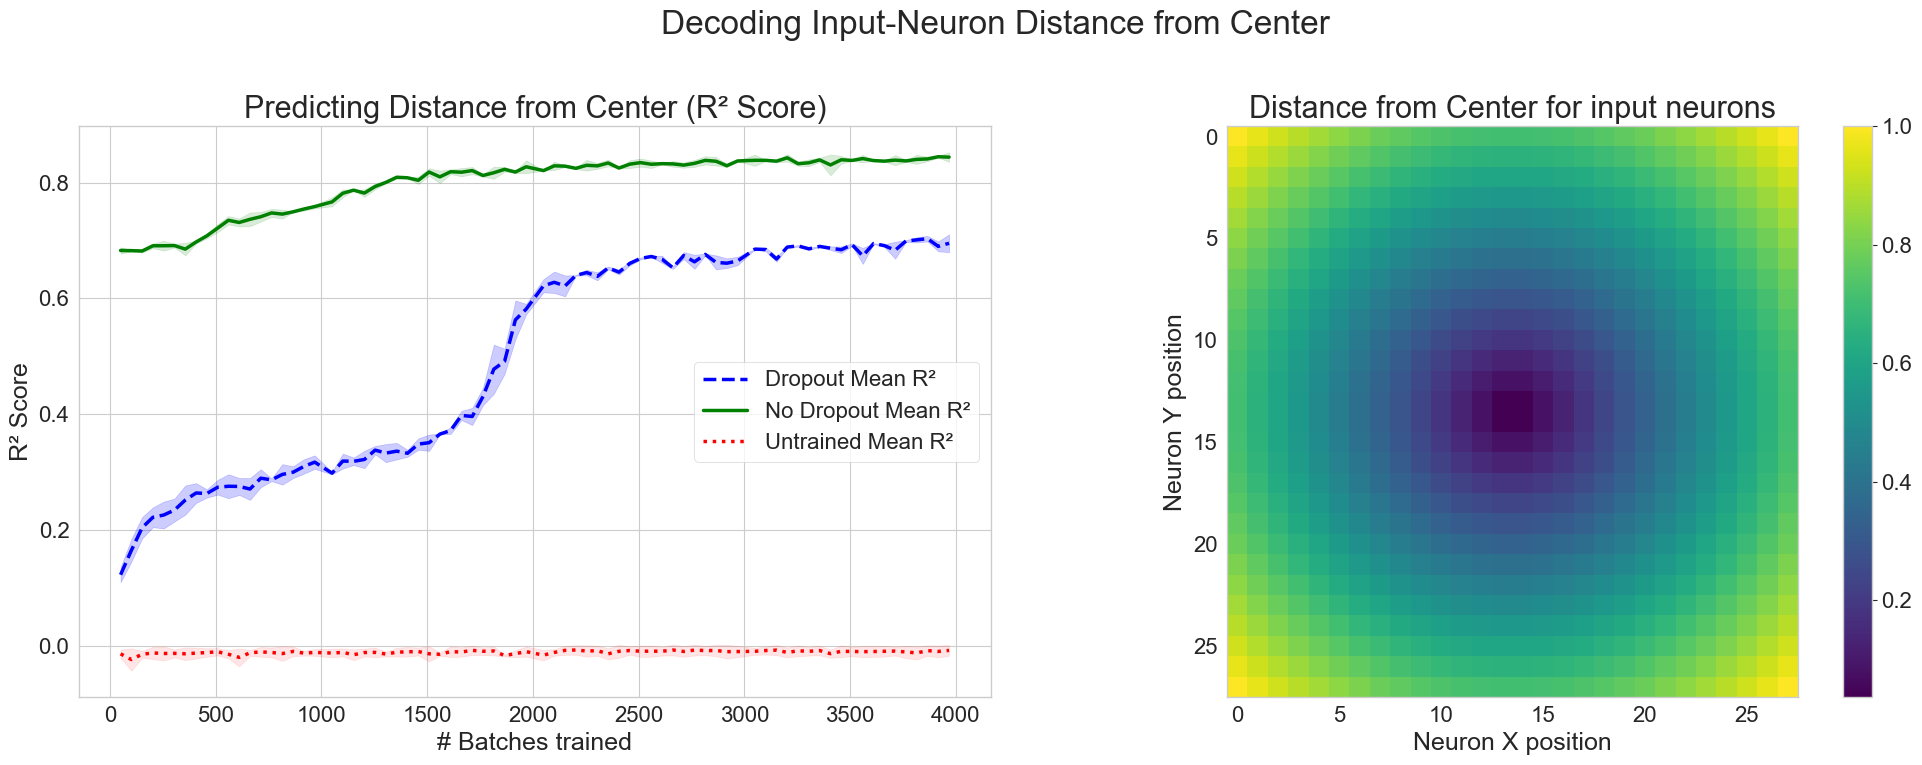
\includegraphics[width=0.8\textwidth]{figures/input-neuron-distance-prediction-accuracy.png}
\caption{Input neuron distance prediction accuracy across different training paradigms for predicting pixel distance from center based on relational structure.}
\label{fig:input-accuracy}
\end{figure}

Analogous to Exhibit 1, we probe whether the decoder exploits the entire relational geometry or merely the target neuron's local neighbourhood by feeding it only the cosine-similarity row corresponding to that neuron.

\begin{figure}[htbp]
\centering
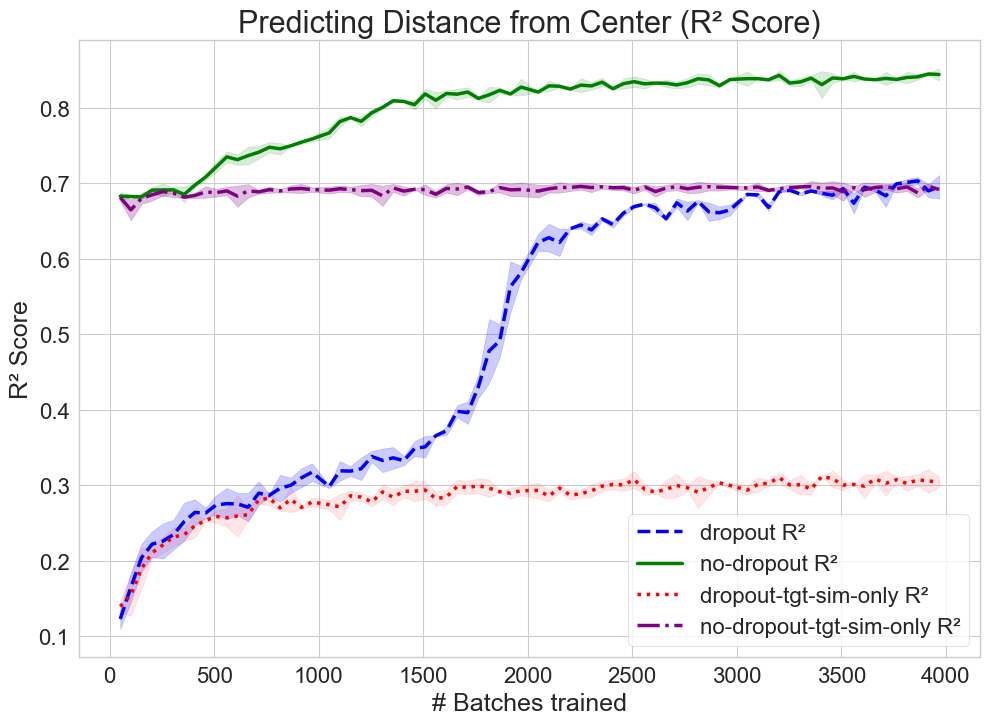
\includegraphics[width=0.8\textwidth]{figures/target-similarity-only-input-pixels.png}
\caption{Target similarity only for input pixels: Performance comparison when using only local neighborhood information versus full relational structure. The decoder can extract useful information from local neighborhoods, but adding more relations significantly improves performance.}
\label{fig:target-similarity-input}
\end{figure}

We can see that, while the decoder can indeed extract useful information solely from the local neighborhood of the target neuron, adding more relations significantly improves performance. This validates our intuition that a richer relational structure helps in disambiguating a representation.

Next, we assess how the size of the relational graph that we provide to the decoder affects the decoding accuracy. To do this, we sample uniformly random subsets of the 784 input neurons and perform the decoding task on the relational structure of subsets of varying sizes.

\begin{figure}[htbp]
\centering
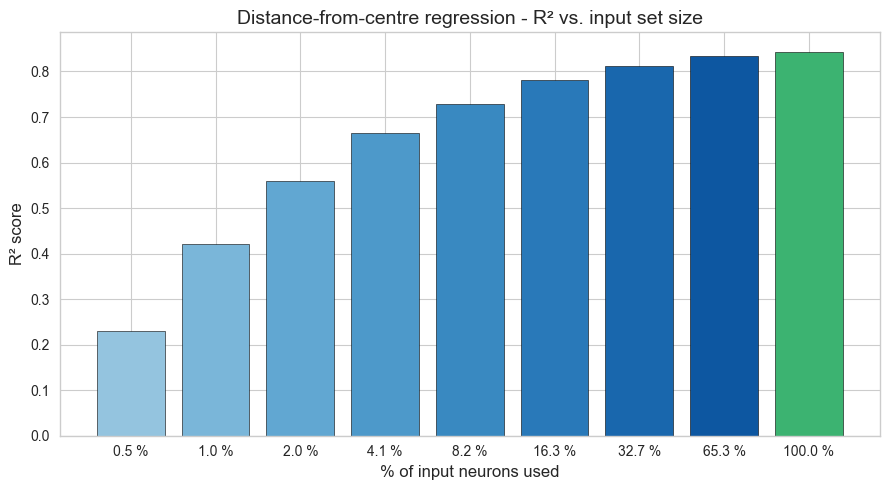
\includegraphics[width=0.8\textwidth]{figures/varying-subset-size-input-pixels.png}
\caption{Varying subset size for input pixels: Distance-from-centre regression R² vs. input set size. Performance improves as we increase the size of the relational graph provided, with diminishing returns at larger sizes.}
\label{fig:varying-subset}
\end{figure}

We can see that, while performance improves as we increase the size of the relational graph provided, adding more neurons to the input yields diminishing returns at some point. In other words, intentional content can be extracted from neurons even when considering only a subgraph of the relational structure they are embedded in.

\section{Model Accuracy and Representational Ambiguity}

We showed that a decoder can be trained to recover representational content by looking at a set of relations between neurons. To link this more directly to the concept of \emph{ambiguity}, we want to return to the idea discussed in our definition of ambiguity.

We defined representational ambiguity as $H(I|R)$: the entropy over all possible interpretations that remain once the representation $R$ is fixed. Empirically, however, we never wield a ``God's eye'' universal decoder. Every decoder we train is built for a specific task context. We denote this context by $C$.

Because $C$ is already baked into the trained decoder, the quantity we can bound in experiments is:

\begin{equation}
H(I|R,C)
\end{equation}

the entropy that remains given both the relational structure encoded in $R$ and the contextual constraint that interpretations must come from the known label set defined by $C$.

\subsection{Ambiguity-Reduction Score (ARS)}

We define:

\begin{equation}
\text{ARS} = 1 - \frac{H(I|R,C)}{H_{\max}}
\end{equation}

where $H(I|R,C)$ is the conditional entropy of interpretations $I$ given a representation $R$ under the same context $C$ as the task, and $H_{\max}$ is the entropy of a completely ambiguous representation ($\log_2 K$ for $K$ classes; $h(Y)$ for a continuous target $Y$).

ARS $\approx 0$ means the representation is maximally ambiguous; ARS $\approx 1$ means it is fully unambiguous.

\subsection{Lower-bound from accuracy (classification)}

Fano's inequality links top-1 accuracy $A$ to entropy:

\begin{equation}
H(I|R,C) \leq h_b(1-A) + (1-A)\log_2(K-1)
\end{equation}

where $h_b(p)$ is the binary entropy function $h_b(p) = -p\log_2(p) - (1-p)\log_2(1-p)$, which measures the uncertainty of a binary random variable with probability $p$. This yields the bound we report:

\begin{equation}
\boxed{
\text{ARS} \geq 1 - \frac{h_b(1-A) + (1-A)\log_2(K-1)}{\log_2 K}
}
\quad (K=10 \text{ for MNIST})
\end{equation}

Note: Since the bound relies only on top-1 accuracy, treating every mistake as if any of the other $K-1$ classes could be correct, it overestimates residual ambiguity, so the reported ARS values are conservative lower bounds.

\subsection{Lower-bound from R2 (regression)}

Assuming Gaussian residuals and standardizing the target so $\text{Var}(Y) = 1$,

\begin{equation}
H(Y|R,C) \leq \frac{1}{2}\log_2(2\pi e(1-R^2))
\end{equation}

which leads to

\begin{equation}
\boxed{
\text{ARS} \geq \frac{\log_2[1/(1-R^2)]}{\log_2(2\pi e)}
} \approx \frac{\log_2[1/(1-R^2)]}{4.094}
\end{equation}

\subsection{Experimental Results}

For Exhibit 1 (class-ID decoding using Gram matrix matching):

\begin{center}
\begin{tabular}{lcc}
\toprule
Training Paradigm & Position Accuracy & ARS (lower bound) \\
\midrule
Dropout & 1.000 & 1.000 \\
No Dropout & 0.383 & 0.122 \\
Untrained & 0.120 & 0.001 \\
\bottomrule
\end{tabular}
\end{center}

For Exhibit 2 (pixel-distance regression using self-attention decoder):

\begin{center}
\begin{tabular}{lcc}
\toprule
Training Paradigm & $R^2$ & ARS (lower bound) \\
\midrule
Dropout & 0.695 & 0.419 \\
No Dropout & 0.844 & 0.654 \\
Untrained & -0.008 & 0.000 \\
\bottomrule
\end{tabular}
\end{center}

\section{Discussion}

We demonstrated that networks trained on MNIST encode class identity of output neurons relationally in their output weights. The learned decoder achieved 75\% accuracy, while geometric matching reached 100\% accuracy for dropout networks. Training paradigm affects the strength of relational encoding, with dropout producing more distinctive geometries.

Perfect decoding accuracy indicates $H(I|R) = 0$: complete determination of representational content by relational structure. Our experiments formally measure $H(I|R,C)$ where $C$ represents context. While this conditioning on $C$ might seem to impose significant limitations, there are reasons to believe these reflect practical rather than fundamental constraints on relational decoding approaches.

The dataset classification results demonstrate that key components of $C$ can be inferred from $R$ itself. We achieve near-perfect accuracy (0.998) distinguishing MNIST from Fashion-MNIST networks based solely on relational structure, showing that task domain (a major component of $C$) is actually encoded in $R$. This suggests that the distinction between $I$ (content to be decoded) and $C$ (context) is somewhat artificial and arises only because our decoder operates in a limited domain. $C$ could be viewed as part of $I$ that we simply choose not to decode in our experimental setup. The results point toward the possibility of approaching true $H(I|R)$ rather than just $H(I|R,C)$—a universal decoder trained on relational structures in larger, multi-modal neural networks could potentially eliminate the need for explicit context conditioning, requiring at most a very broad context consisting of our part of the universe and choice of modalities. Additionally, cross-architecture transfer results suggest that network architecture might not be a crucial component of the context.

These results demonstrate a practical approach for operationalizing the ambiguity measure $H(I|R)$ in neural representations. Higher decoding accuracy corresponds to lower conditional entropy, providing a quantitative framework for measuring representational ambiguity. The perfect geometric matching results for dropout networks show that relational geometry alone can unambiguously specify representational content in a given context.

This suggests that neural networks can achieve the low-ambiguity representations that theoretical accounts of consciousness require. This methodology extends naturally to other representational domains, offering a path toward both empirically measuring the ambiguity of representations and directly decoding their content across different neural systems.

\section{Related Work}

\subsection{The Platonic Representation Hypothesis}

Huh et al.'s mutual k-NN kernel-similarity, originally applied to large cross-modal models, is also closely linked to decoder accuracy (and thus ambiguity reduction) in our small MNIST networks \cite{huh2024}. Here, we compute the metric by comparing the weights of output neurons across MNIST networks trained with different seeds. This relationship suggests that, if the pattern holds, higher kernel-similarity should indicate lower representational ambiguity even in larger, multimodal settings.

\begin{figure}[htbp]
\centering
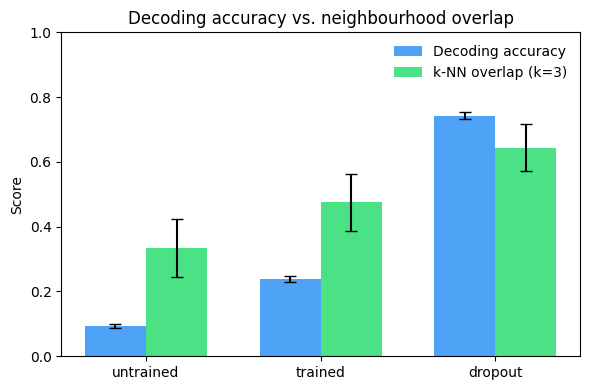
\includegraphics[width=0.8\textwidth]{figures/knn-kernel-similarity-vs-decoder-accuracy.png}
\caption{kNN Kernel Similarity vs. Decoding Accuracy: Relationship between Huh et al.'s mutual k-NN kernel-similarity metric and our decoder accuracy measurements, suggesting a connection between representational alignment and ambiguity reduction.}
\label{fig:knn-similarity}
\end{figure}


\bibliographystyle{unsrt}
\bibliography{references}


\end{document}